% Set up the document
%\documentclass[a4paper, 12pt, oneside]{bThesis} % My own class, based on the report class
%\documentclass[a5paper, 10pt]{bThesis} % Looks more like a book
%\documentclass[b5paper]{bThesis} % Looks more like a book
%\documentclass{bThesis} % Plain
\documentclass[oneside]{bThesis} % Plain
%\documentclass[a5paper,DIV=12,BCOR=9mm,headsepline,headings=small,cleardoubleempty,10pt]{bThesis} % Settings from Open Advise

% Info
\author{J\'on Bergmann Maronsson}
\title{The Glory of Non-Extremal Stationary Points\pending}

% Paths
\graphicspath{{figures/}}

% Start the document
\begin{document}

% The preamble stuff
% Titlepage
\begin{titlepage}
%\vspace{2cm}
%\noindent{\bf University of Iceland \\ Faculty of Natural Sciences \\ Department of Chemistry} \\ 
%\noindent \HRule \vspace{10mm}

%\begin{center}
%{\LARGE \bf Theoretical Calculations of }\\
%\vspace{3mm}
%{\LARGE \bf Electrochemical Systems }\\
%\vspace{8mm}
%\normalsize{by}\\
%\vspace{5mm}
%\large{ \bf J\'on Bergmann Maronsson}\\ \vspace{27mm}
%\includegraphics[width=45mm]{hi} \\ \vspace{27mm}
%\normalsize{ Thesis for the degree of  \\ Magister Scientiarum in Chemistry \\ October 2008}
%\end{center}
%
%\HRule
%
%\noindent \textbf{Thesis Advisor: Professor Hannes J\'onsson}\\
%\noindent \textbf{Co-Advisor: Associate Professor Yoshitada Morikawa }\\
%\noindent \textbf{External Examiner: Professor Vi\dh{}ar Gu\dh{}mundsson }

\maketitle

\end{titlepage}


% Flyleaf
%\begin{titlepage}
% \hspace{10cm}
%\end{titlepage}

% Set the page count for the preamble
\pagestyle{plain}
\pagenumbering{roman}
\setcounter{page}{2}

% Include the preamble
\section*{Preface}
\addcontentsline{toc}{chapter}{Preface}

This thesis is submitted in candidacy for the Ph.D. degree from the Technical University of Denmark (DTU).
The work has been carried out between November 2008 and February 2012 at the Ris\o{} DTU campus, formerly the Ris\o{} National Laboratory for Sustainable Energy, DTU; the Center for Atomic-scale Materias Design (CAMd) and with external stays at the University of Iceland.
The project was supervised by Tejs Vegge from the Technical University of Denmark and co-supervised by Hannes J\'onsson from the University of Iceland.
The project's funding was provided by \expand

\vspace{10mm}
\begin{flushright}
Kgs. Lyngby, February 29th 2012,\\

\vspace{15mm}

\rule{50mm}{0.1pt}\\
\textit{J\'on Bergmann Maronsson}
\end{flushright}

\newpage
\chapter*{Abstract}
\addcontentsline{toc}{chapter}{Abstract}

Reaction rates in theoretical chemistry was the main focus of this thesis.
Applying current methods to aid analysis of experimental data in complex borohydrides and improving these commonly used methods.

Complex borohydrides are materials of high hydrogen storage capacity and too high thermodynamic stability.
Understanding the high stability is of great importance to the development of suitable materials for hydrogen storage.
In an effort to gain insight into the structural transitions of two such materials, \ce{Ca(BH4)2} and \ce{Mg(BH4)2}, low temperature rotational dynamics experiments were performed.
The work presented here revolved around assisting in the data analysis by performing density functional theory calculations on the possible dynamical events.
For the \ce{Mg(BH4)2}, only rotational dynamics were detected and they were in good agreement with the experimental values, showing that $C_2$-type rotations happen at lower temperatures than $C_3$-type rotations and that approximately $15\%$ of the \ce{BH4} units activate at a lower temperature than the rest.
For the \ce{Ca(BH4)2}, in addition to the rotational dynamics, longer range diffusion was detected.
Most likely this was due to \ce{H2}-interstitial defects.
The rotational dynamics were more prominent in the data and good agreement with the experiments was reached, showing that $C_3$-type rotations activate at lower temperatures than $C_2$-type rotations.

A method for finding the ridge between first order saddle points on a multidimensional surface was developed.
For atomic scale systems, such points on the energy surface correspond to atomic rearrangement mechanisms.
Information about the ridge can be used to test the validity of the harmonic approximation to transition state theory for reaction rates,
in particular to verify that second order saddle points - maxima along the ridge - are high enough compared to the first order saddle points.
Furthermore, corrections to the harmonic approximation can be estimated by direct evaluation of the configuration integral along the ridge.
New minima along the ridge can also be identified during the path optimisation,
thereby revealing additional transition mechanisms.
The method is based on modifying the gradient of a set of points along a path connecting the saddle points to iteratively converge to the ridge.
%The method is based on optimising a string of discretisation points along a path between the saddle points and using an iterative optimisation which requires only the force acting on the atoms.
At each iteration during the optimisation, the gradient is inverted along an unstable eigenmode perpendicular to the path, effectively mapping the ridge to a minimum energy path.
The method was applied to Al adatom diffusion on the Al(100) surface to find the ridge between 2-, 3- and 4-atom concerted displacement
and hop mechanisms for diffusion.

\newpage
% Rename the Icelandic abstract
%\renewcommand{\abstractname}{\'Agrip}
%\begin{abstract}
%\TH{}etta er frekar magna\dh{}.
 
%\end{abstract}
% Restore the abstract to English

%\begin{center}
%\section*{}
%\vspace{20mm}
\section*{Resum\'e}
\addcontentsline{toc}{chapter}{Resum\'e}

%\selectlanguage{danish}

Forståelse af reaktionshastigheder er en essentiel del af moderne forskning på atomar skala.
I denne afhandling beskrives anvendelsen af veletablerede metoder til beskrivelse af vigtige hydrogenlagrings-systemer. Herefter videreudvikles metoderne for at kunne opnå en bedre beskrivelse af reaktionsvejsomgivelserne, for herigennem at bestemme reaktionshastigheden med større nøjagtighed.

Komplekse borohydrider er materialer med en høj hydrogenlagrings-kapacitet og er yderligere meget termodynamisk stabile (for stabile til hydrogen lagring).
For at få bedre indsigt i de strukturelle overgange i to sådanne materialer, \ce{Ca(BH4)2} og \ce{Mg(BH4)2}, blev der udført lav-temperatur rotationsdynamik eksperimenter.
%(I am actually not sure what you mean excactly when talking about structural transitions, but I think this translation should suit most of it :-) furthermore I am not sure whether "rotationsdynamik" is the correct word to use - I do not know much (anything) about it.. so you should probably ask an expert :-) )
Arbejdet der præsenteres her omhandler assistance i forbindelse med dataanalyse, ved hjælp af tæthedsfunktionalteori-beregninger, på de mulige dynamiske hændelser.
For \ce{Mg(BH4)2}, var der god overensstemmelse med eksperimenter. $C_2$-type rotationer observeres ved lavere temperaturer end $C_3$-type rotationer og cirka $15\%$ af \ce{BH4}-enhederne aktiveres ved lavere temperaturer end resten.
For \ce{Ca(BH4)2} observeredes, udover rotationsdynamikken, en uidentificeret hændelse, som ifølge beregningerne sandsynligvis skyldes \ce{H2}-interstitielle defekter.
I god overensstemmelse med eksperimenter, aktiveres $C_3$-type rotationer ved lavere temperaturer end $C_2$-type rotationer.

For at undersøge reaktionsvejes omgivelser, blev der udviklet en metode til at finde højderyggen mellem førsteordens saddelpunkter på en multidimensional overflade.
Information om højderyggen kan bruges til at verificere den harmoniske approksimation brugt i forbindelse med transition-state-teorien anvendt til bestemmelse af reaktionshastigheder, specielt i forbindelse med verificeringen af at andenordens saddelpunkter, maksima langs højderyggen, er beliggende højere sammenlignet med førsteordens saddelpunkter.
%(I am not sure whether to use "ryg" or "højderyg" - the last one is used in geology and for describing mountains, whereas the first also simple means back (human's). Is multidimensional surface an OK word, it is only a surface if in 2d?. I do not think we have a Danish word for tst.)
Yderligere kan korrektioner til den harmoniske approksimation estimeres ved direkte evaluering af det konfigurative integerale langs højderyggen.
%(I am not sure about "konfigurative" have never heard about it..)
Nye minima langs højderyggen kan også identificeres sideløbende med reaktionsvejs-optimeringen, og derigennem kan yderligere transitions-mekanismer afsløres.
Metoden er baseret på modifikation af gradienten, for et sæt af punkter langs reaktionsvejen der forbinder saddelpunkterne, så den iterativt konvergerer mod højderyggen.
Ved hver iteration under optimeringen, inverteres gradienten langs en ustabil egentilstand vinkelret på reaktionsvejen. Dette afbilder effektivt højderyggen mod en minimum reaktionsvej, som kan findes med flere forskellige kendte teknikker.
Metoden blev anvendt til at studere Al adatom diffusion på Al(100) overfladen, for at finde højderyggen mellem en samlet bevægelse af 2, 3 eller 4 atomer, samt hoppe-mekanismer i forbindelse med diffusion.
Der var signifikante korrektioner for samlet bevægelse af 3 og 4 atomer. 
%(I am not sure if adatom is OK in Danish...)
Højderyg-metoden er en enkel metode som kan anvendes til at verificere reaktionshastigheder, men har potentialet for at bestemme mere nøjagtige hastigheder i sig selv, ved at repræsentere transition-state med højderyggen.



%\selectlanguage{english}

\newpage 
\chapter*{Acknowledgements}
\addcontentsline{toc}{chapter}{Acknowledgements}

\placeholder
%\begin{itemize}
% \item Professor Hannes J\'onsson, at the University of Iceland, for his guidance and inspiration.
% \item Associate Professor Yoshitada Morikawa, at the University of Osaka, for his guidance and kind manner while I was in a strange culture.
% \item Egill Sk\'ulason for collaboration, discussions and proof-reading.
% \item The members of the J\'onsson research group, at the University of Iceland, for enlightening discussions and support:
% \begin{itemize}
%  \item Sigr\'i\dh{}ur Gu\dh{}mundsd\'ottir, also for proof-reading
%  \item J\'on Steinar Gar\dh{}arsson M\'yrdal
%  \item Andreas Pedersen
%  \item Jean-Claude Berthet, Ph.D.
%  \item Peter Kl\"upfel, Ph.D.
% \end{itemize}
% \item The members of the J\'onsson research group, at the University of Iceland, for help with compilation issues, discussions and proof-reading:
% \begin{itemize}
%  \item Andri Arnaldsson, Ph.D.
%  \item Finnbogi \'Oskarsson
% \end{itemize}
% \item The members of the Yoshida research group, at the University of Osaka, for discussions, help and kind acceptance in a strange culture:
% \begin{itemize}
%  \item Susumu Yanagisawa, Ph.D.
%  \item Ikutaro Hamada, Ph.D.
%  \item Kunihiko Yamauchi, Ph.D.
% \end{itemize}
%% \item The best curry place in existence, Senba Curry, at the train station at Kita-Senri in Osaka, Japan.
% \item Friends and family for putting up with my studies for such a long time.
% \item Computer facilites: Bj\'olfur, J\"otunn and Itanium
% \item Funding:
% \begin{itemize}
%  \item Japanese Government (MONBUKAGAKUSHO:MEXT) Scholarship
%  \item Science Institute of the University of Iceland
% \end{itemize}
%\end{itemize}


% Tables of contents
\tableofcontents
%\listoffigures
%\listoftables

% Abbreviations
%\newpage
%TST - Transition State Theory

HTST - Harmonic Transition State Theory

SP - Saddle Point

\sap{1} - First Order Saddle Point

\sap{2} - Second Order Saddle Point

\sap{N} - $N$th Order Saddle Point

DFT - Density Functional Theory

%\newpage

% Reset the page count for the main content
\newpage
\pagestyle{plain}
\pagenumbering{arabic}
\setcounter{page}{1}


% Input the main parts
\part{Introduction}
\label{part:introduction}
\chapter{Introduction}
\label{chap:introduction}

\bit
%\item Stationary Points in general
%\item Finding extrema
%\item Other sorts of stationary points
%\item Minima in theoretical chemistry
%\item Saddle points in Chemistry (reaction rates)
\item Why do we want to find higher order saddle points in chemistry.
\item Energy storage, conversion and mobility (Hydrogen as an example)
\item The importance of assessing reaction rates (Kinetics is a very important aspect for the above)
\item General problems with getting reaction rates
\item Annoying landscapes
\item Beyond harmonicity
\item The methods for finding stationary points presented here are inspired by chemistry but are applicable to any function.
\item The thesis is heavily biased towards chemistry
\eit

The border between mathematics, physics and chemistry is often times fuzzy and the methods developed for one may very well benefit the others (for example \expand \citemiss).
Common to all, is some form of functional analysis where the study of stationary points\footnote{Points where the first derivative is zero.} is generally of great interest.
For systems of limited dimensionality, finding stationary points becomes no more complex than solving a root problem for the function's derivative.
However, once systems grow beyond a few dimensions, solving the root problem becomes infeasible.
Furthermore, the lack of a global analytical function \tred{(Is analytical correct in this context?)} makes it impossible to simply solve for the roots.
This is, generally, the case in atomistic simulations, which is the main subject of this thesis.
While the methods discussed herewithin are developed in this field, applying them to purely mathmatical problems and within other fields is mearly a question of implementation, thus they are presented as general as possible in order to appeal to wider audiences.

Locating extrema using local information, i.e. the gradient, is a well known technique\citemiss, whereas the gradient is simply followed in the appropriate direction (positive for maxima and negative for minima) until it vanishes.
Finding other stationary points is less obvious and classifying them depends on the second order derivatives (or even higher in special cases\footnote{e.g. the Monkey Saddle \url{http://mathworld.wolfram.com/MonkeySaddle.html}})
Finding such points without explicitly evaluating higher order derivatives is an important subject within atomic simulations, since their calculation is is very costly when using non-analytical \tred{(Is QM technically non-analytical and what is the exact definition of analytical?)} models to describe the atomic interaction.

\subsubsection{Significance of Stationary Points in Atomic Simulations}
The potential energy of atomic systems can be evaluated as a function of the atomic coordinates.~\cite{born-oppenheimer-1927, schrodinger-equation-1926, kohn-1999}
The interesting features of such a mapping are generally considered to be the minima which represent stable configurations of the atoms.
The transition between minima is then considered to be a chemical reaction.
These can range, for example, from rotations of specific groups with minimal impact on the properties of the material (\fref{chap:borohydrides}) and motion of water molecules in liquid water~\citemiss to adsorption~\citemiss and the breaking of strong chemical bonds~\citemiss.
In understanding the transition in question, the path of least resistance (or minimum energy path) is an essential concept, since the highest point along it defines the potential energy that must be overcome.
This point is a non-extremal stationary point (i.c. first order saddle point) and information about the frequency of a given transition (its reaction rate) can be inferred from from it and its surroundings, which is of central importance in chemistry.\cite{htst-wert-1949, htst-vineyard-1957}

\subsubsection{Old Methods Introduction}
The focus of this thesis is the application of theoretical methods to calculational reaction chemistry.
The underlying methods that allow this are numerous and their discovery span ages in time, from Newton's equations of motion~\cite{newton-latin} up to modern day methods for solving Sch\"odinger's equation~\cite{schrodinger-equation-1926} for quantum systems\cite{hohenberg-kohn-1964, gpaw-review-2010}, from the discovery of calculus\citemiss\footnote{see Leibnitz: \url{http://books.google.dk/books?id=UdGBy8iLpocC&pg=PA46&redir_esc=y\#v=onepage&q&f=false}} and vector math~\citemiss to modern methods for solving eigenvalue problems\citemiss.
%This chapter will give a brief look at the main methods employed with special emphasis on those that constitute the basis of the novel method presented in \fref{chap:erm}.

Simulations of atomic systems are an integral part of modern atomic scale research, whether it be to investigate specific electronic structure properties\citemiss, performing atomic dynamics\citemiss or investigating macroscopic properties\citemiss.
Simulations are commonly employed in the analysis of interesting material properties (see for example catalytic properties\citemiss), the screening of candidate materials --- to eliminate the need to synthesize as many unsuccesful materials --- for various processes (see for example hydrogen storage\citemiss) and further collaboration and comparison with experiments (see for example \citemiss).

Reaction chemistry happens on a timescale of microseconds which is, essentially, eternity when seen from the vantage point of the fast moving vibrations, which happen on a timescale of femtoseconds.
Briding this gap is an important research subject which remains open, despite noble efforts that have moved the field a long way\citemiss.

%Dating back to well before modern large scale computer clusters, synamical studies were even performed using tools no more complicated than balls, sticks, pens and paper~\cite{old-simulations-bernal-1962} ATH: Vegetable Staticks (Stephen Hales, 1727)


%\tblue{The order of the topics for discussion in this chapter is still a bit off.
%Born-Oppenheimer is needed before TST but it should be introduced at the same (similar) time as the Schr\"odinger equation which in turn should accompany the DFT section (close to which the potential function section should lie).}
%\bit
%\item Perhaps use the Newton/Schr\"odinger figure I made a bit back (modified if needed)
%\item General on atomistic simulations (seguing to potential functions and DFT)
%\item Why statistical methods
%\item Why path techniques (introduction to be expanded on in the TST section)
%\item It is now "possible" to do long timescale MD simlations but statistical methods are still more suited to find "all" the processes (chat with Elvar on MD)
%\item (Why these methods but not some other?)
%\item Methods that or of particular interest get better coverage.
%
%\item Would be nice to have a figure of each of the main guys for each methodology
%\bit
%\item Born, Oppenheimer
%\item Hesse
%\item Arrhenius, Kramer
%\item Hannes, Graeme
%\item Hohnberg, Kohn
%\eit
%\eit


%\section{Notation}
%\bit
%\item Nuclei positions: $\vR$
%\item Electron positions: $\vr$
%\item R-basis for formulas
%\item The PES: $E(\vR)$
%\item Gradient vs. Force
%\eit

\subsubsection{Chapter Outline}
\label{sec:chapters}

\fref{chap:methods}: Methods
\fref{chap:borohydrides}: Metal Borohydrides ...
\fref{chap:erm}: Beyond Harmonicity
\fref{chap:al}: Self-Diffusion of Aluminium ...
\fref{chap:perovskites}: Coupled Hydrogen Defects ...




\part{Theoretical Methods}
\label{part:theory}
\chapter{Methods}
\label{chap:methods}
%\section{Introduction}
\label{sec:methods-introduction}

% ------------------------------------------------------------------
\bit
\item Perhaps use the Newton/Schr\"odinger figure I made a bit back (modified if needed)
\item General on atomistic simulations (seguing to potential functions and DFT)
\item Why statistical methods
\item Why path techniques (introduction to be expanded on in the TST section)
\item (Why these methods but not some other?)
\eit

\placeholder

\chapter{Traversing Potential Energy Surfaces}
\label{chap:pes}

This chapter introduces the idea of potential energy surfaces (PESes) and discusses their creation and exploration.

\incomplete

\input{chapters/methods/schrodinger}
\input{chapters/methods/born-oppenheimer}
\input{chapters/methods/dft}
\input{chapters/methods/potential-functions}
\input{chapters/methods/force}
\input{chapters/methods/optimisers}
\input{chapters/methods/hessian}
\input{chapters/methods/saddle-points}
\input{chapters/methods/paths}

\section{Transition State Theory}
\label{sec:tst}
% ------------------------------------------------------------------

Transition State Theory (TST) is a formalism dedicated to providing reaction rates in a purely theoretical setting where running dynamical trajectories of the required length is infeasible.

\incomplete

\subsection{Motivation}

\subsubsection{The Time-scale Problem}

\figmiss{Timescale problem (I have one somewhere, just need to polish it and stick it in)}

In atomistic simulations there is a often a clear separation of timescales between the most interesting events.
With local vibration of the atoms being very fast, typically on the order of $10^{14} \unit{Hz}$~\citemiss,
while non-local reordering of atoms, motion between minima on the PES, often considered as rare-events, typically occur on the order of $10^3 \unit{Hz}$ for a system with an energy barrier of $0.5 \unit{eV}$.~\citemiss
Depending on the temperature of the system, a tremendous amount of calculations (on the order of $10^10$) would have to be performed to have a reasonable probability of seeing each rare-event while also fully modelling the details of the atomic vibrations.

Even though performing dynamics long enough to accurately describe both types of events, is technically possible~\citemiss, e.g. by minimising vibrations to allow for longer timesteps~\citemiss or modifying the PES~\cite{hyperdynamics-voter-1997}, the key to long-timescale dynamics still lies outside the reach of such methods as they spend most of their time performing dynamics that are not of particular interest for molecular dynamics.
This is true, in particular, for calculations that rely on costly, but accurate, quantum calculations and/or large systems.

In the problem lies also the solution, when there is such a clear separation of time-scales, it is possible to treat the problem with statistical methods.
Essentially dealing with the vibrational areas of the PES (the basins) by averaging over them and seperately locating ares of transitions.

\subsection{The Basics}

\subsubsection{Assumptions}
There are four main assumptions made within TST, which vary in severity.
\paragraph{Born-Oppenheimer}
The Hamiltonian of the system can be separated, resulting in a single PES for the trajectories.
\paragraph{Classical Dynamics}
No tunnelling or other quantum effects --- apart from those offered by the calculational method of the PES --- are taken into account in the vanilla TST.
The motion of the system is governed by classical dynamics.
Quatnum effects are included in extensions to TST (see for example \cite{qtst-hj-1997, qtst-hj-1998, qtst-hj-2009}~\citemiss) but this is not relevant to the work presented in this thesis and will not be discussed further.
\paragraph{Thermal Equilibrium}
The system will spend considerable time in each basin of the PES, long enough such that the Boltzmann distribution for ... can be employed.
For systems with large energy barriers in comparison with the thermal energy~\footnote{A rule of thumb is that $E_\text{b} > 5\kB T$~\citemiss}, this assumption holds well but for smaller barriers or high temperatures it breaks down as thermal equilibrium becomes difficult to achieve and the separation of timescales is lost
\paragraph{No Re-Crossings}
Once the system has left a basin, it does not return for a significant amount of time (long enough to thermalise in the new basin).
This assumption is the most serious and efforts to minimise its effects are discussed below.

\subsubsection{The Transition State}

\figmiss{Transition State}

When dividing the phase space (position and momentum) into two areas, reactants (R) and products (P), a hypersurface separating the two emerges.
This hypersurface is referred to as the transition state ($\ts$)\footnote{The dagger, $\ts$, is a conventional symbol for the transition state} and represents a bottleneck region which each reactive trajectory crosses on its way from R to P.
Commonly, momentum is disregarded in the definition of the phase space, which is then  $3N$ dimensional, within which the $\ts$ is a $3N-1$ dimensional subspace.

\subsubsection{Statistical Methods}

\bit
\item Configuration Integrals (or partition functions?)
\eit

Take advantage of the time-scale separation ...

TST aims at overcoming the time-scale problem by way of "averaging" over the fast vibrational motion to present a reaction rate for the rare-events.

Boltzmann distribution...
Maxwell distribution (velocity)...

%The partition functions require the total energy of the $N$ atoms system,
%\beq{tst-total-energy}
%E(\vR, \vect{v}) = V(\vR) + \frac{1}{2} \sum_i^{N} m_i \left| \vect{v}_i \right|^2
%\eeq
%with atoms at $\vR$ with velocity $\vect{v}$, travelling on the PES, $V$.

\incomplete

The most important assumption remains, any trajectories that cross the TS do not recross it.
This assumtion is also the weakest link \expand

\subsection{Reaction Rates}
The reaction rate, $k^\text{TST}$, is defined as the probability of being at the $\ts$,
%$P_\ts = \langle \delta(\vR - \vR_\ts) \rangle_\text{R}$,
\beq{ts-probability-partition-simple}
P_\ts = \frac{Z_\ts}{Z_\text{R}},
\eeq
thermally averaged over R, with velocity away from R,\citemiss
\beq{tst-rate-initial}
k^\text{TST} = \frac{1}{2}|\vect{v}_\perp| P_\ts,
\eeq
where $\vect{v}_\perp$ is the velocity component perpendicular to the $\ts$ and the factor $1/2$ comes from the fact that only half of the trajectories will be moving away from R.
Due to the different dimensionality of the $\ts$ and R, $P_\ts$ isn't strictly a probability as it has the unit $\unit{m^{-1}}$. \expand

The velocity at each point $\vR$ can be taken from a Maxwell distribution, \tred{(Why is this okay?)}
\beq{tst-maxwell-velocity}
\langle |\vect{v}| \rangle = \sqrt{\frac{2kT}{\pi m}},
\eeq
where $m$ is the mass of the particles \tred{(This is wrong)}.
The rate then becomes
\beq{tst-rate-full}
k_\text{TST} = \sqrt{\frac{kT}{2\pi m}} \frac{Z_\ts}{Z_\text{R}}. \quad \text{\expand}
\eeq

\placeholder

\subsubsection{Optimisation of the Rate}
\bit
\item Dynamical Recrossings
\item Variational TST
\item Search for the true TS
\eit

The choice of the TS is essential for an accurate rate.
In fact, due to the assumption of no recrossings, TST offers a variational way to discover the true rate,
\beq{tst-variational-rate}
k^\text{TST} \ge k^\text{exact},
\eeq
where the transition state is the variational parameter.

\subsubsection{Quantum TST}
\bit
\item If a short introduction with citations is possible.
\item No long discussion on QTST.
\eit

\subsubsection{Assumptions Revisited}
Discuss the implications of the assumptions.
\bit
\item Born-Oppenheimer
\item Classical Dynamics (No tunnelling)
\item Thermal Equilibrium (Boltzmann)
\item No recrossings (Most severe and the reason for the variational property of the TS???)
\eit
\placeholder

%\subsubsection{Misconception???}
%A prevailant misconception regarding TST is that there is an "activated complex" that every rare-event becomes before moving to the product state
%
%\placeholder

\subsection{Methods for Metadynamics}
\bit
\item Some references here would be nice but \tblue{not a priority}.
\item Hyperdynamics
\item AKMC
\eit
\placeholder


\subsection{Harmonic Transition State Theory}
\label{sec:htst}

% ------------------------------------------------------------------

\placeholder

\subsubsection{Terminology ("Transition State" vs. "Saddle Point")}
Due to the popularity of the harmonic approximation to TST, a common misconception is that saddle points and transition states are interchangeable terms.
This is apparent in the literature, even where HTST is directly discussed or saddle points and reaction paths found.
\tblue{No need to "name and shame"?}

The confusion stems from the fact that the saddle point is the only geometrical feature needed to construct the transition state.
Once found, the saddle point acts as the ... \tblue{Write after the actual definition of HTST has been written out.}

Even though the distinction is not overly important within HTST, it is of central importance in TST, as the actual definition of the transition state is vital.

\recent

\incomplete
 % subsection from TST
\section{First Order Saddle Point Methods}
\label{sec:sps}

Finding saddle points is a non-trivial task in multiple dimensions, when only local information is available.

\incomplete

% ------------------------------------------------------------------
\subsection{Nudged Elastic Band}
\label{sec:neb}

Finding Steepest Decent Paths (SDPs) from a given point is simple by following the gradient with a small stepsize.
On the other hand, finding specific SDPs that end at minima is not.
The goal here is to find two SDPs each leading from the same \sap1 to different minima without any further information than the minima.


\incomplete

% ------------------------------------------------------------------
\subsection{Dimer}
\label{sec:dimer}

The Dimer method was inspired by Voter\cite{voter-hyperdynamics-1997}

Given only an initial point, $\vR$, on a multidimensional function, $F(\vR)$, the goal is to, iteratively, locate a nearby \sap1, using no direct calculation of the Hessian, i.e. using only functional values and the first derivatives.
Indiredct information about the Hessian is, however, used in the form of an estimate of the eigenmode corresponding to its lowest eigenvalue (minimum mode).
Using the minimum mode, $\uvn$, it is possible to locally transform \sap1s to minima and using conventianl techniques to move up-hill to locate the \sap1.

The dimer method can be split into three independant phases.
\ben{dimer-phases}
\item Estimating the minimum mode.
\item Transforming the gradient to make \sap1 seem as minima.
\item Translating the point according to the transformed gradient.
%\item Invert the gradient components that lie parallel to the minimum mode and translating system.
\een

\subsubsection{Minimum Mode Estimation}
A pair of points (the dimer), $[\vR_\text{A}, \vR_\text{B}]$, are chosen, close to current point $\vR_0$, such that
\beq{dimer-separation}
\vR_\text{A} = \vR_0 + \Delta_\text{D}\uvn \quad \text{and} \quad \vR_\text{B} = \vR_0  - \Delta_\text{D}\uvn
\eeq
where $\Delta_\text{D}$ is a predefined constant to determine the length of the dimer.

Rotating the dimer around its central point, $\vR_0$, until $F(\vR_\text{A}) + F(\vR_\text{B})$ is minimized yields a good estimate of the lowest curvature direction and thus the minimum mode. \cite{voter-hyperdynamics-1997}
The manner in which this rotation is performed is varied...

%% Need to introduce the gradient as a symbol first....
%Often $F(\vR_0)$ has either been evaluated or needs to be.
%This can be taken advantage of as this neccesary calculation can be used to extrapolate values for one of the end points.
%To illustrate this $F(\vR_0)$ and $F(\vR_\text{A})$ have already been calculated.
%The value at $\vR_\text{B}$ can then be extrapolated,
%\beq{dimer-extrapolate}
%F(\vR_\text{B}) = 2F(\vR_0) - F()
%\vR_\text{}
%\vR_\text{}
%\vR_\text{}
%\vR_\text{}
%\vR_\text{}
%\vR_\text{}
%\eeq

\incomplete

\subsubsection{Gradient Transformation}
Once a minimum mode estimate is available for the current point, $\vR_0$, it is possible to transform the gradient so that any \sap1 is transformed to a minimum.
\beq{dimer-transform}
\nabla{}F(\vR_0)
\eeq

\tblue{This latter step is not unique to the dimer algorithm... Lancoszs...}

\incomplete

\subsubsection{Iterative Translation}

\incomplete

%\section{Potential Functions}
\label{sec:potentials}

\bit
\item Introduce pairwise potentials
\item Quickly discuss EAM/EMT
\eit

%\section{Quantum Calculations}
\label{sec:methods-QM}

With increased computing power and, in particular, advances in parallel algortims, it is now possible to calculate a range of physical properties for materials on the atomic level without the use of any experimental parameters.
Such \textit{ab initio} (from the beginning) methods ...
\expand

\subsection{The Electronic Structure Problem}
The Schr\"odinger equation is the quantum analoge of Newton's equations of motion and thus governs the motions of the quantum system in question as well as its observables.
\expand

The Born-Oppenheimer approximation (\fref{sec:born-oppenheimer}) allows the separation of the Hamiltonian to an electronic part and a nuclear part.
Thus, the positions of the nucleii, $\vR_I$ only enter the calculations as parameters.
A full quantum treatment will not be discussed here.
\expand

A non-relativistic system of $N$ electrons (and $N_I$ nuclei) is described by the time independant Schr\"odinger equation,
\beq{schrodinger-basic}
 \widehat{H}\Psi = E\Psi,
\eeq
where $\Psi \equiv \Psi(\vr_1, \vr_2, ... ,\vr_N)$ is the wave function, depending on the spatial coordinates, $\vr_i$, of each electron, $E$ is the electronic energy of the system and $\widehat{H}$ is the hamiltonian,
\beq{hamiltonian}
\widehat{H} = -\sum_i^N \frac{\nabla^2_i}{2} - \sum_i^N \sum_{j>i}^N \frac{1}{\left| \vr_i - \vr_j \right|} - \sum_i^N \sum_I^{N_I} \frac{1}{\left| \vr_i - \vR_I \right|} + V_\text{ext},
\eeq
which consists of 4 terms.
First there is the kinetic energy of the electrons, then the electron-electron interaction, followed by the electron-nuclei interaction and finally any external influence (e.g. an applied electric field) is represented by a single term.

Though it may look innocent, solving the Schr\"odinger equation is a daunting task and in most cases significant approximations must be made.

\subsection{Density Functional Theory}
\label{sec:methods-dft}

One of the most popular and common teqchniques for solving the electronic structure problem is the Density Functional Theory (DFT) which can, from first principles (\textit{ab initio}), exactly (in theory) solve the Schr\"odinger equation.
However, in practice, approximations must be made for all but the most simple systems.
Nevertheless, DFT has produced many interesting and good results and is now a well established formalism that is continually being reviewed and improved.
Furthermore, the \textit{ab initio} nature of DFT makes it a great companion to experimental research, not only for comparison and prediction of interesting materials but also to assist and expand upon data analysis.
%The founding father of DFT is Walter Kohn who received the Nobel Prize in chemistry for his development of the density functional theory \cite{kohn1999} in 1998 along with John Pople who received the prize for his development of computational methods in quantum chemistry \cite{pople1999}.

\subsubsection{The Hohenberg-Kohn Theorem}
According to the Hohenberg-Kohn (H-K) theorem there is a one-to-one correspondence between the wavefunction and the electron density of the ground state. Once this has been established, it is simple to see that the total energy is a unique functional of the electron density, $\rho(\textbf{r})$, which is an observable while the wavefunction is not,
\begin{equation}
\label{eq:H-KenergyDensity}
 E[\rho] = \langle \Psi[\rho] | \widehat{H} | \Psi[\rho] \rangle.
\end{equation}
The Raleigh-Ritz variational principle is used to minimize the energy and find the ground state and density, %[missing ref]
\begin{equation}
 E_{0} = \min_{\rho(\mathbf{r})} \left(E[\rho(\mathbf{r})] \right).
\label{eq:H-Kvariational}
\end{equation}
This is the basis of DFT, developed by Hohenberg and Kohn \cite{hohenberg1964} in 1964.

\subsubsection{The Kohn-Sham Equations}
Currently there is no known way to perform the one-to-one mapping suggested by the H-K theorem. However in 1965 Kohn and Sham (K-S) published an indirect approach for calculating the energy functional $E[\rho]$ \cite{kohn1965}.
They showed that the interacting many-electron system can be mapped, approximately, onto a non-interacting system of single electron states, $\{\phi_i\}$, where each electron is subject to the effective potential $v_{eff}(\vect{r})$ due to all other particles. These one electron wavefunctions can be produced by solving the K-S equations,
\begin{equation}
\label{eq:K-Sequation}
 \left\{-\frac{1}{2} \nabla ^2 + v_\mathrm{eff}(\vect{r}) \right\} \phi_i(\vect{r}) = \epsilon_i \phi_i(\vect{r}).
\end{equation}
Since both the effective potential and the wavefunctions are unknown these equations must be solved self-consistently.
The electron density can then be produced using the square of the wavefunctions,
\begin{equation}
\label{eq:electronDensity}
 \rho(\vect{r}) = \sum_{i=1}^N \left| \phi_i(\vect{r}) \right|^2.
\end{equation}
The effective potential can be written as
\begin{equation}
\label{eq:effectivePotential}
 v_\mathrm{eff}(\vect{r}) = v(\vect{r}) + v_{H}(\vect{r}) + v_{XC}(\vect{r})
\end{equation}
where $v(\vect{r})$ is the sum of the potential due to the kinetic and ionic parts in equation \ref{eq:generalHamiltonian}%[Is this correct and do I need to include this reference]
, $v_{H}(\vect{r})$ is the Hartree potential,
\begin{equation}
\label{eq:hartreePotential}
 v_{H}(\vect{r}) = \int d^3r \frac{\rho(\vect{r'})}{\left| \vect{r} - \vect{r} \right|},
\end{equation}
and
\begin{equation}
\label{eq:XCpotential}
 v_{XC}(\vect{r}) = \frac{\delta E_{XC}[\rho]}{\delta \rho(\vect{r})}
\end{equation}
is the potential due to the exchange-correlation functional, $E_{XC}[\rho]$, which will be discussed in section \ref{sec:XCfunctional} 

\subsubsection{The Exchange-Correlation Functional}
\label{sec:XCfunctional}
The Kohn-Sham equations are in principle exact, however the exchange-correlation functional, $E_{XC}[\rho]$, is generally not known and has to be approximated. The accuracy of the approximation becomes a major issue in solving the Kohn-Sham equations.

The exchange-correlation functional is a local functional which describes the electron-electron interaction,
\begin{equation}
\label{eq:XCfunctional}
 E_{XC}[\rho] = \int d^3r\, \epsilon_{XC}(\rho, \vect{r})\rho(\vect{r})
\end{equation}
where $\epsilon_{XC}(\rho, \vect{r})$ is the exchange-correlation energy density.

The approximations used in our work are based on the so-called Generalized Gradient Approach (GGA). The GGA uses the the exchange-correlation energy of a homogeneous electron gas at point $\vect{r}$ like the Local Density Approximation (LDA) \cite{kohn1965} but also uses the gradient of the density to account for inhomogeneity. This, however, is not a good choice by itself so a reduced density gradient, $s(\vect{r})$, is used, as suggested by Langreth and Perdew \cite{langreth1977}. The exchange-correlation functional then becomes
\begin{equation}
  E_{XC}^{GGA}[\rho] = \int d^3r\, \epsilon_{XC}^{GGA}(\rho(\vect{r}), s(\vect{r}))\rho(\vect{r})
\end{equation}
with
\begin{equation}
\label{eq:GGAreducedDensityGradient}
 s(\vect{r}) = \frac{\left|\nabla \rho(\vect{r})\right|}{2\sqrt[3]{3\pi^2\rho(\vect{r})} \rho(\vect{r})}.
\end{equation}
%The calculations in chapter \ref{ch:japan} use GGA based on the PBE functional \cite{perdew1996} while the calculations in chapter \ref{ch:dacapo} use GGA based on the RPBE functional \cite{hammer1999}.

\subsection{Implementation of DFT}
\label{sec:methods-dft-implemetnation}

\subsubsection{The Plane Wave Basis Set}
In implementing DFT calculations, the Kohn-Sham wavefunctions are expanded in a particular basis set. In our work plane waves are used under periodic boundary conditions in accordance with Bloch's theorem,
\begin{equation}
\label{eq:blochsTherom}
 \psi_\vect{k}^{m}(\vect{r}) = \sum_\vect{G}c_{\vect{k} + \vect{G}}^m\, e^{i(\vect{k}+\vect{G})\cdot\vect{r}}
\end{equation}
where $\vect{G}$ are the reciprocal lattice vectors. %[what are $c_{\vect{k} + \vect{G}}^m$?]. 
For an exact solution, an infinite number of plane waves is needed. Fortunately the plane waves at the lower end of the kinetic energy range are the most important, so the number of plane waves can be reduced by defining a cutoff, $G_{cut}$, where the solution becomes good enough:
\begin{equation}
 \left( \frac{\hbar^2}{2m} \right) \left| \vect{k} + \vect{G}_{cut} \right|^2 \le E_\mathrm{cut}.
\end{equation}
This leads to one of the main advantages of plane waves. By increasing the cutoff the accuracy of the calculation can be systematically increased. 

A disadvantage of plane waves is their inefficiency to deal with high curvature regions, such as the atomic core. To overcome this pseudopotentials can be used. In the core, pseudopotentials are an average of the potential due to the core electrons and the nucleus felt by the valence electrons inside a given sphere but outside the sphere the pseudopotential becomes identical to the all-electron potential. The plane-wave cutoff can be lowered even further when using pseudopotentials while generally giving results of good accuracy, especially the so-called ultrasoft pseudopotential with non-local components \cite{vanderbilt1990}.



\part{Thesis Proper \pending Discussion?} 
\label{part:thesis}
\chapter{Complex Borohydrides}
\label{chap:borohydrides}
\section{Introduction}
\label{sec:borohydrides-introduction}

%\bit
%\item Order/Disorder transitions
%\item Difficult to get atomic level experimental data (emphasize), thus, calclations important to help
%\item Kinetically limited processes
%\item Multiple phases
%\item Structures are not fully known (but mostly)
%\item Large superstructures
%\item Reading this chapter should give an overview of the theoretical work performed but for a full discussion, refer to the respective papers.
%\eit

With high hydrogen density, both volumetric (up to \missing{}~\citemiss) and gravimetric (up to \missing{}~\citemiss), metal borohydrides are of tremendous interest as mobile hydrogen storage candidates.
However, they commonly exhibit poor reversibility~\citemiss, slow ab- and de-sorbtion kinetics~\citemiss and too high thermodynamic stability~\citemiss.
Understanding these drawbacks is an important research subject in order to solve them or discover new, better, materials for hydrogen storage.

The work presented here\footnote{and in full detail in papers \ref{pap:calcium} and \ref{pap:magnesium}} is focussed on detecting and understanding atomic scale hydrogen motion in two species, \ce{Mg(BH4)2} and \ce{Ca(BH4)2} --- which have shown lower thermodynamic stability than other borohydrides~\cite{borohydride-stability-2006, calcium-stability-2006}, e.g. \ce{LiBH4}, while still having high hydrogen density ($14.9\%\text{wt}$ and $11.5\%\text{wt}$, respectively) and showing partial reversibility~\citemiss --- in order to better understand structural transition and decomposition mechanisms.
Out of the possible hydrogen dynamics, rotations of borohydride groups are easily overlooked as uninteresting but they are often associated with order-disorder phase transitions in coordination compounds.~\cite{order-disorder-2006, order-disorder-2010}
Furthermore, longer range diffusion of hydrogen or \ce{BH4} could be part of the decomposition mechanism.
Atomic level experimental data for these types of dynamics is scarce and experimental methods are limited to a handful of techniques, one of which is quasielastic Neutron Scattering (QENS), which is sensitive to hydrogen motion~\cite{qens-bee-1988} on the range of interest and have, to some extent, been used to study interstitial metal hydrides for other species.~\citemiss

Due to the scarcity of appropriate experiments, collaboration between experimental and theoretical researchers is essential to fully interpret and understand their results.
For some of the borohydrides the unit cells are very large and hard to deal with on the theoretical level.
This is well illustrated by the fact that the exact structure of the cells is still in active refinement in the literature.~\cite{cabh42-structure-p42m, cabh42-structure-p4}
The existence of multiple phases can complicate matters even further as their local geometry may be similar.~\citemiss [32-38 in paper \ref{pap:magnesium}]
However, for the work presented here, only a single phase was present.

%Metal borohydrides and other complex hydrides have not recieved as much attention in the literature.
%\expand



\section{Co-operation Between Theoretical and Experimental Work}
\label{sec:cooperation}

% ------------------------------------------------------------------
\placeholder

\section{Calcium Borohydride [$\beta$-\ce{Ca(BH4)2}]}
\label{sec:borohydrides-calcium}

\ben
\item Calculate rigid rotations of \ce{BH4-} to get a "feel" for the landscape
\item Then calculate the reaction paths (MEPs) and saddle points
\item Prepare HTST rates and compare with experiments
\item Revise the experimental rates as applicable
\item Do further MEP calculations for mechanisms that still remain unexplained in the experimental data
\een

\placeholder

\section{Magnesium Borohydride [$\beta-$\ce{Mg(BH4)2}]}
\label{sec:borohydrides-magnesium}

%\bit
%\item Calculate rigid rotations of \ce{BH4-} to get a "feel" for the landscape for all the different borons in the cell
%\item Show multiple PESes
%\item Then calculate the reaction paths (MEPs) and saddle points
%\item Prepare HTST rates and compare with experiments
%\item Flat landscape $\rightarrow$ Introduce the next section
%\eit

The calculational supercell was relaxed, from the $fddd$ spacegroup ($\#70$), totalling 176 atoms.
The structure consists of 5 symmetry inequivelant \ce{BH4} sites which all have similar local structure, being wedged between 2 \ce{Mg} atoms (\fref{fig:mg-local-structure}).
The symmetry inequivilance stems from the fact that each \ce{BH4} was slightly away from the \ce{Mg}-\ce{Mg} axis.
The distance, $L$, from the \ce{B} to the axis, influences the barriers.

\figmiss{Environment, for explaining the axes used}

The experimental data detected only rotational diffusion.
Thus, the work exclusively revolved around understanding which rotations correpsonded with the experiments.

For each inequivelant site a number of rigid rotation PESes were constructed in order to get an overview of the interesting events and to limit computations spent on the MEP calculations, similar to \fref{sec:borohydrides-calcium}.
Due to symmetry not all the axes needed to be considered.

The general result from the PESes was that rotations that maximised the \ce{Mg}-\ce{H}, $d_{H-Mg}$ distance showed the lowest energies (\fref{fig:h-mg-distances}).
In this respect, two distinct types of $C_2$ axes were seen, those parallel to the \ce{Mg}-\ce{Mg} axis, $C_2^\parallel$, which maximised $d_{H-Mg}$ and those perpendicular to it, $C_2^\perp$, where $d_{H-Mg}$ was generally lower and had higher barriers.
MEP calculations for the latter found a combination of other axes yielded the same permutation but at a much lower energy cost.
The difference in relative barrier height decreased with decreasing $L$.\footnote{The relative difference would be non-existant for $L=0$ but non of the \ce{BH4} fulfill that critrion.}

\begin{figure}[h]
\begin{center}
  \subfigure[Average \ce{H}-\ce{Mg} distance]{
    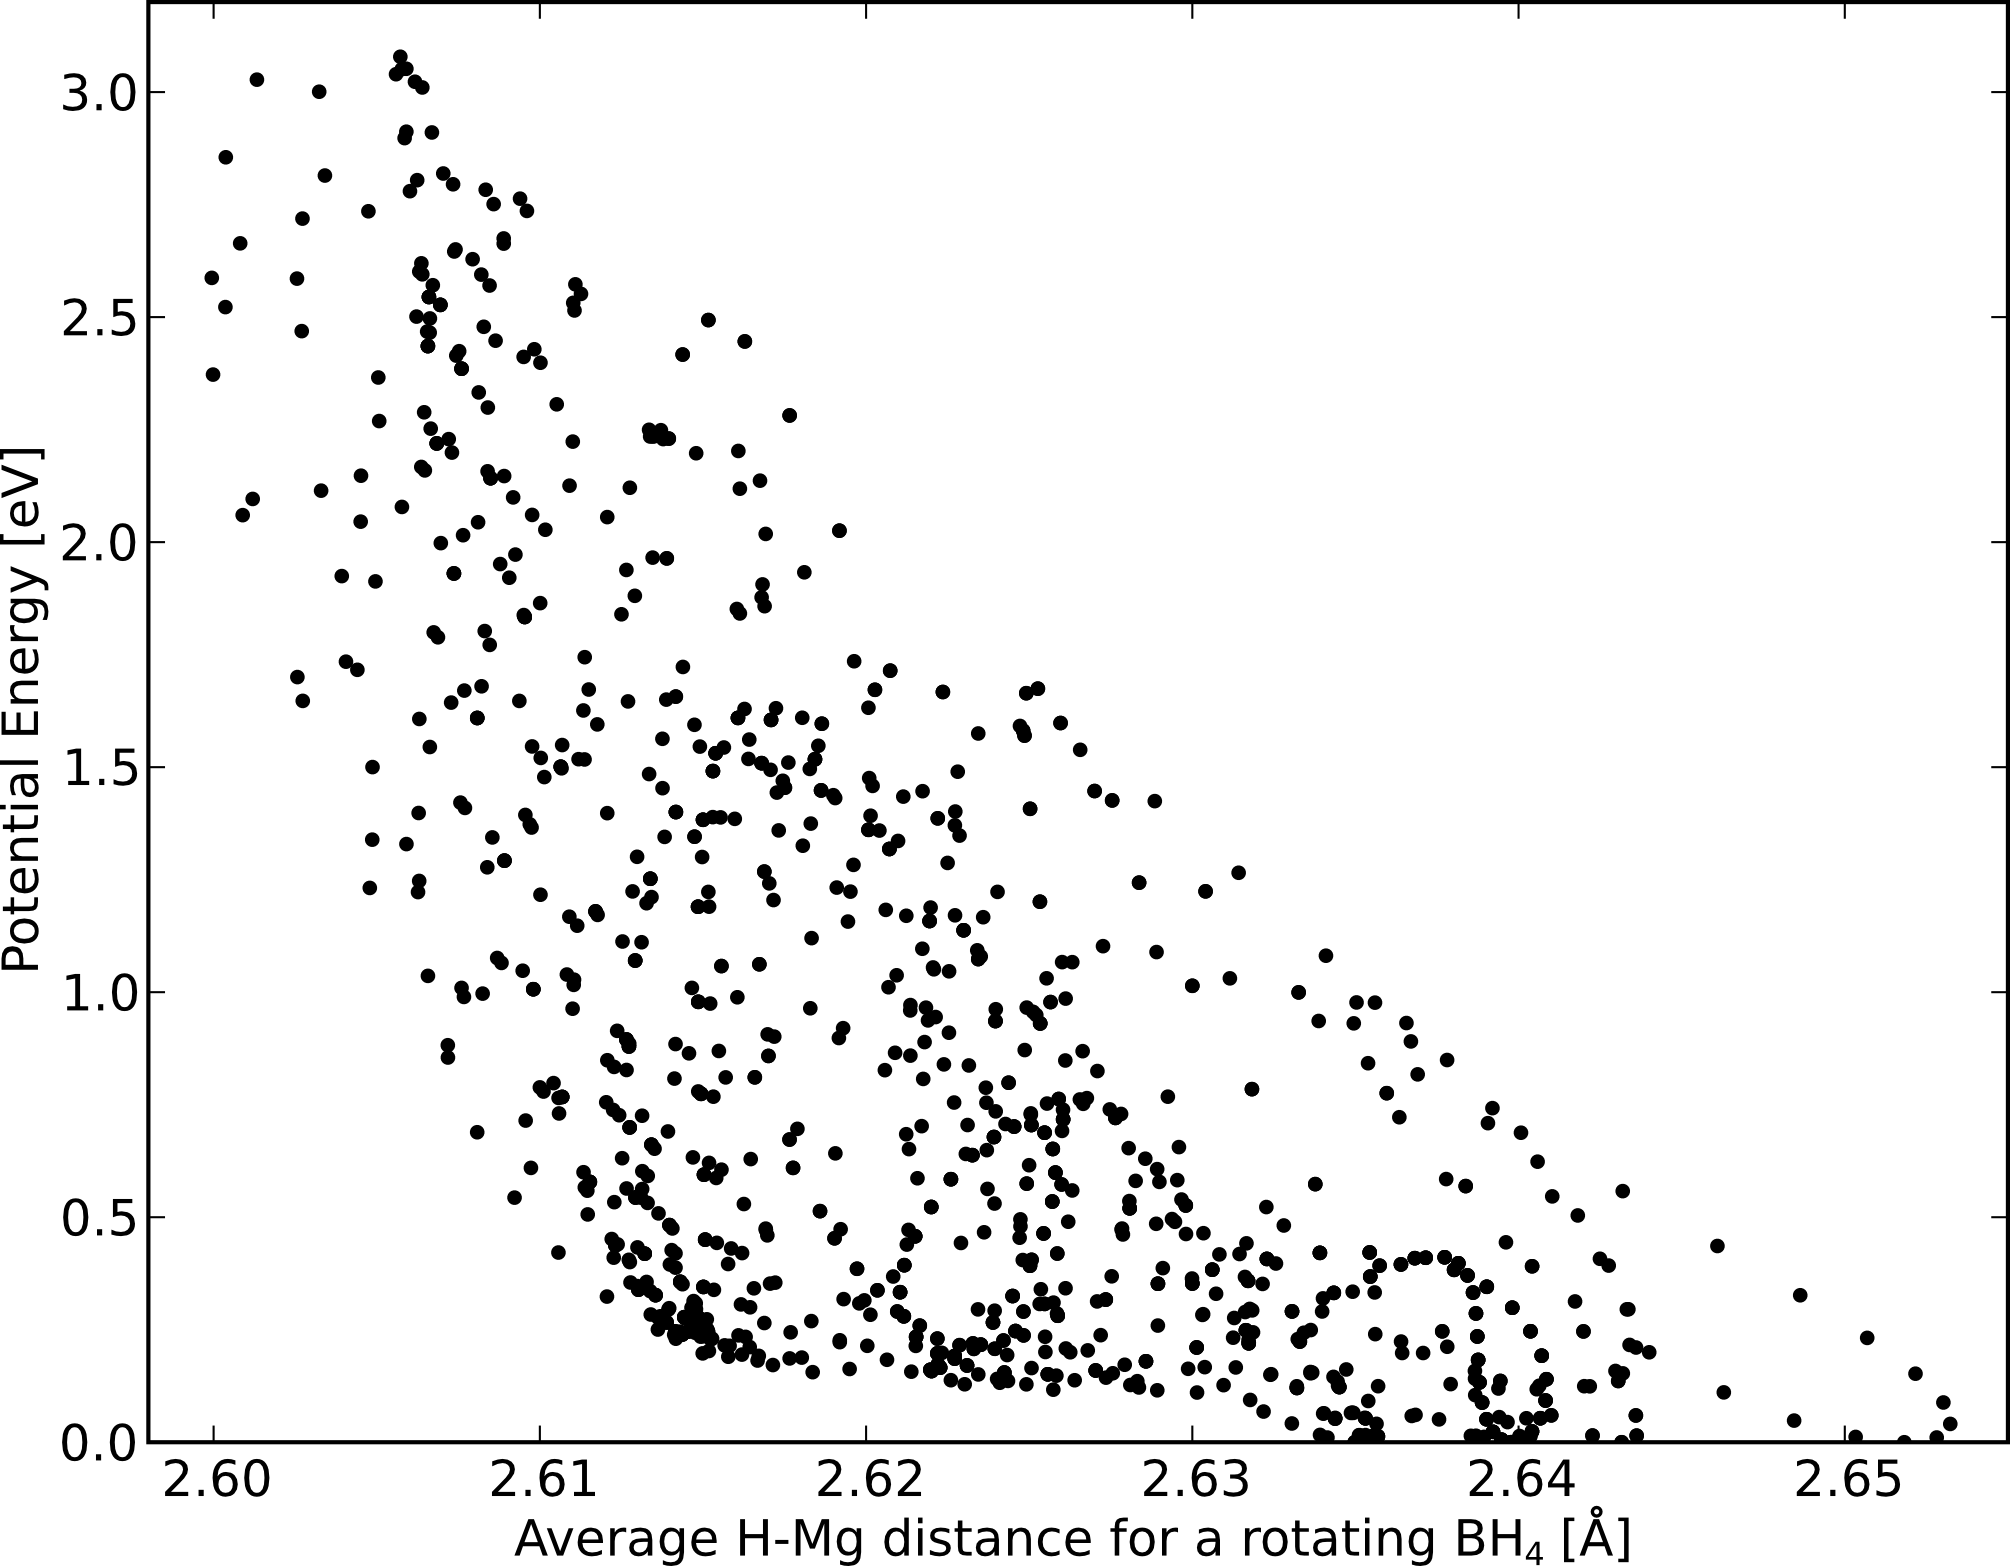
\includegraphics[width=0.45\linewidth]{h-mg-distances-avg}
    \label{fig:h-mg-distances-avg}
    }
  \subfigure[Minimum \ce{H}-\ce{Mg} distance]{
    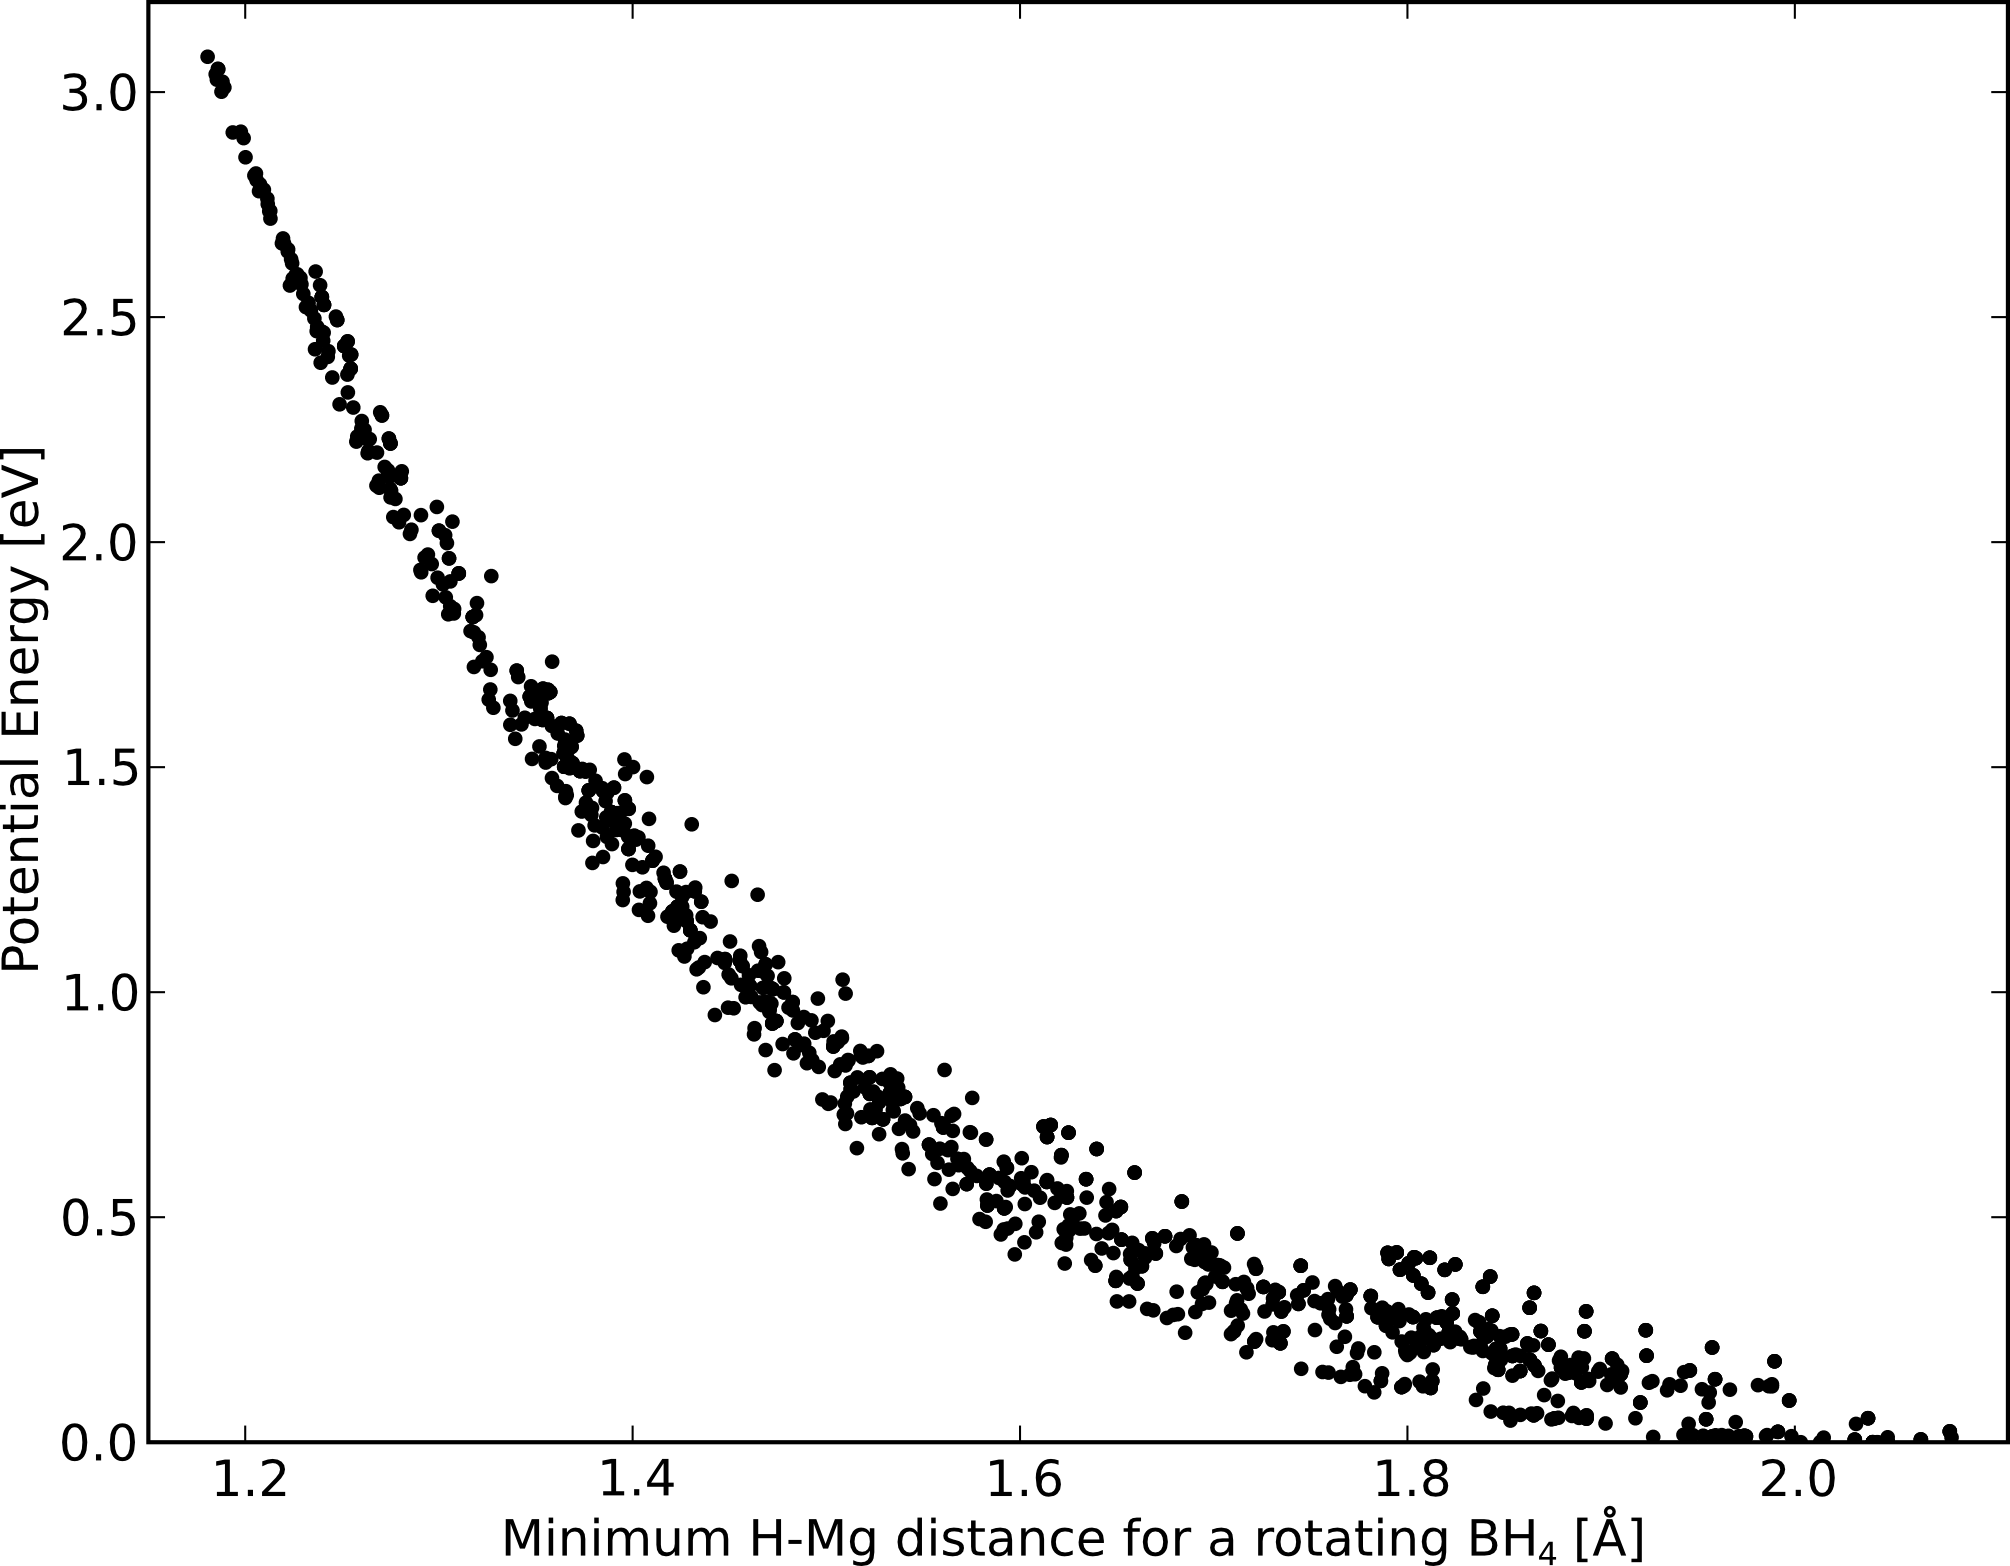
\includegraphics[width=0.45\linewidth]{h-mg-distances-min}
    \label{fig:h-mg-distances-min}
    }
    \parbox{0.85\linewidth}{
      \caption{For each PES, the distances between the \ce{H} atoms of the rotating \ce{BH4} unit to the neighboring \ce{Mg} atoms is plotted.
Some systemaitc features can be seen since the data was produced with specific rotations rather than a uniform distirubtion.
A clear trend for lower energies with higher distances can be seen.
      }
      \label{fig:h-mg-distances}
    }
\end{center}
\end{figure}

\figmiss{The different gengeral types of PESes.}

No such clear distinction could be made with regards to the $C_3$ axes.
However, due to symmetry all the $C_3$ axes for a given site yield a very similar PES. \tblue{(Should I show the four PESes for B04?)}

The rigid rotation plots are not able to give a full description of the events, neither their geometry nor their energetics.
Thus MEP calculations were performed with the lowest energy rigid rotation paths as starting guides.
The barriers from 

\figmiss{Barrier dependancy on distance}

It is unsurprising to find that there is a direct relationship between $L$ and the $C_2$ barrier height.
In fact, the relationship is linear, as can be seen in \fref{fig:mg-barriers}, with increased $L$ the barrier increases which is most likely due more \ce{H}-\ce{Mg} interaction.
On the other hand, no such direct relationship could be found for the $C_3$ axes.

\incomplete


\chapter{Energy Ridge Mapping}
\label{ch:erm}
\section{Introduction}

A ridge is a colloection of steepest decent paths (SDPs) between any \sap2s and \sap1s between two end \sap1s.

We shall first introduce the finding of ridges for any given function of multiple variables before taking the specific example of potential energy surfaces (PESes) and atomic simulations and,
finally, investigating the quality of HTST in \tblue{2 systems}:
The diffusion of Al on an Al(100) surface and \tblue{...}.

\incomplete

\section{Energy Ridge Profiling}
PLACEHOLDER

\section{Testing}
\label{sec:erm-testing}
% ------------------------------------------------------------------

\placeholder



\chapter{Self diffusion of aluminium}
\label{chap:al}
\section{Introduction}
\label{sec:al-introduction}
An Al adatom on the Al(100) surface provides an interesting system to study because several different low energy diffusion mechanisms have been found, including various concerted displacements of two or more atoms, in addition to the, more intuitive, hop mechanism~\cite{concerted-motion-1990, dimer-original-1999, ts-opt-2001}.
The dimer method, on which the current implementation of ridge calculations heavily depends, has been used successfully on the system~\cite{dimer-original}, using the well tuned and fast embedded atom method (\fref{sec:potentials})~\cite{eam-1983, eam-1986}.
This made the system an excellent candidate for trying the newly implemented ridge method (\fref{chap:second-order}, paper \ref{pap:second-order}).

The obvious hop-over-ridge ($E_\text{b} = 0.372\unit{eV}$) is not the lowest energy diffusion mechanism.
Considerably lower in energy is the concerted motion of 2 atoms, where the adatom burrows into the surface to replace an atom which in turn pops out of the surface at a neighbouring site.
This mechanism has a barrier of $E_\text{b} = 0.227\unit{eV}$.
Related to the concerted 2 atom mechanism are the concerted 3 atom ($E_\text{b} = 0.426\unit{eV}$) and concerted 4 atom ($E_\text{b} = 0.413\unit{eV}$) mechanisms, where more surface atoms take part in the concerted mechanism.
These latter diffusional mechanisms are of a noticeably longer range than the hop --- and to a lesser extent the concerted 2 atom mechanism --- as the surface atom that "pops" up, does so in a more distant site.

Of course, there is an incredible amount of mechanisms possible for the 385 atom system of 771 degrees of freedom\footnote{The calculational cell was composed of $2$ frozen layers and $4$ free layers of $8\times 8$ atoms with a single adatom on top. For further calculational parameter, please refer to paper \ref{pap:second-order}.}.
However, only these lowest ones were considered for the current study.

The long-range concerted mechanisms are difficult to locate due to their environment being very flat, thus investigating the ridges lying close by is an interesting subject, with a high possibility of seeing low energy \sap{2}s in the vicinity of the \sap{1}s.
Furthermore, there is a clear separation in geometry between the hop mechanism on the one hand and the concerted displacements on the other, giving a similar situation as the one presented in \fref{sec:borohydrides-summary}.

\section{Energy Ridges}
\label{al-energy-ridges}

The energy ridges between all the lowest energy \sap{1}s were calculated.
Two situations of particular interest arose.
The first was the discovery of intermediate \sap{1}s, while the second concerned the HTST reaction rate, its accuracy and efforts to improve it.

\subsubsection{Intermediate \sap{1}s}
\begin{figure}[hp]
\begin{center}
\includegraphics[width = 1.0\linewidth]{discovery}
\caption{
Calculated path at the ridge between the \sap{1}s for a hop and concerted 4-atom displacement.
The circles show the position of converged images (coloured circles for \sap{1}s and \sap{2}s, but grey for the rest). 
These \sap{1}s turned out not to be adjacent on a ridge and the path optimisation reveals an intermediate \sap{1}, the one for the concerted 2-atom displacement.
%This illustrates how a ridge calculation could reveal new and possibly unknown transition mechanisms.
The long path is not able to accurately locate the intermediate \sap{1} and the lower energy \sap{2} due to finite resolution in the discretisation and corner-cutting.
The exact configuration of the \sap{1} can be found using a \sap{1} finding algorithm starting with the approximation obtained from the optimised path.
Then, a calculation of a shorter path, between the \sap{1}s of the 2-atom  and 4-atom displacements, locates the intermediate \sap{2} accurately (cyan circle)
The insets show an overlay of three configurations, two adjacent \sap{1}s and the intermediate \sap{2}.
The atom colours correspond to the coloured spheres of the energy ridge.
}
\label{fig:discovery}
\end{center}
\end{figure}

As can be seen in \fref{fig:discovery} there is a significant energy ridge "barrier" separating the hop and concerted 2 atom \sap{1}s.
More interestingly, ridge calculations between the more populous concerted \sap{1}s (3 and 4 atom) and the hop revealed that they were interspersed with the concerted 2 atom \sap{1}.
This is not surprising as the concerted mechanisms are all quite similar with regards to their coordinates, while the hop mechanism is inherently different.


\subsubsection{Beyond Harmonicity}
\begin{figure}[hp]
\begin{center}
\includegraphics[width = 1.0\linewidth]{low-barriers}
\caption{
The energy ridge going through \sap{1}s of 2-atom, 3-atom, 4-atom and, then the same, 2-atom concerted displacement for an Al adatom on a Al(100) surface.
The circles represent the position of images in the optimised paths, the \sap{1}s and the \sap{2}s being coloured differently but the rest coloured grey.
The green curves represent harmonic approximations to the energy surface at each \sap{1}.
The insets show an overlay of three configurations, two adjacent \sap{1}s and the intermediate \sap{2}.
The atom colours correspond to the coloured spheres of the energy ridge.
}
\label{fig:low-barriers}
\end{center}
\end{figure}
Considering only the simil


\bit
\item 2 concerted "gateway" between hop and other concerted motion.
\eit

\placeholder


\begin{comment}
--- Anything below here is a direct copy from either the \latex file of the manuscript or the online version of the article ---

\section{\label{sec:results-adatom}Application: Al adatom diffusion on an Al(100) surface}

An Al adatom on the Al(100) surface provides an interesting system to study because several different diffusion mechanisms have been found, including various concerted displacements of two or more atoms, in addition to the, more intuitive, hop mechanism~\cite{concerted-motion-1990, dimer-original-1999, johannessson-01}.
An embedded atom method potential (EAM)~\cite{eam-1986} is used here since it has been shown to accurately describe the system and requires much less computational effort than DFT calculations.
The simulated cell was a slab of 6 layers, each of which was $8\times8$ atoms, with one adatom, totalling 385 atoms.
The two bottom layers were kept fixed at bulk positions with a lattice parameter of $4.038\unit{\mAA}$.
Initially, traditional NEB calculations were carried out to find the relevant \sap{1}s which were then used as end points in the ridge calculations.
The spring constant was set at $k = 5.0\unit{eV/\mAA}$.
The two images in the dimer had a fixed separation of $0.0001\unit{\mAA}$ and were allowed to rotate only once for each iteration in the path optimisation.
The initial minimum mode guesses were taken from a Gaussian distribution.
The convergence criteria for the maximum effective force component were set at $0.01\unit{eV/\mAA}$ and $0.001\unit{eV/\mAA}$ for the regular and climbing image calculations respectively.

% Figure 4
\begin{figure}[t]
\begin{center}
\includegraphics[width=0.5\linewidth]{figures/low-barriers}
\caption{
The energy ridge going through \sap{1}s of 2-atom, 3-atom, 4-atom and, then the same, 2-atom concerted displacement for an Al adatom on a Al(100) surface.
The circles represent the position of images in the optimised paths, the \sap{1}s and the \sap{2}s being coloured differently but the rest coloured grey.
The green curves represent harmonic approximations to the energy surface at each \sap{1}.
The insets show an overlay of three configurations, two adjacent \sap{1}s and the intermediate \sap{2}.
The atom colours correspond to the coloured spheres of the energy ridge.
The \sap{2}s adjacent to the 3-atom and 4-atom concerted displacements are low and the harmonic approximation to TST is less accurate for these mechanisms than the 2-atom concerted displacement.
}
\label{fig:low-barriers}
\end{center}
\end{figure}

Several low energy transition mechanisms for adatom diffusion on this surface have been found previously using the dimer method \cite{dimer-original-1999}.
The mechanism with the lowest energy barrier is a two atoms concerted displacement, $E_b = 0.227\unit{eV}$.
The second lowest is the simple hop of the adatom from one site to an adjacent site, $E_b = 0.372\unit{eV}$, but then three and four atoms concerted displacements are only slightly higher in energy $E_b = 0.426\unit{eV}$ and $E_b = 0.413\unit{eV}$.

The potential energy ridges and \sap{2}s were calculated between each pair of \sap{1}s and the results are shown in \fref{fig:low-barriers} for the three concerted displacement mechanisms.
Low energy \sap{2}s were found near the concerted 3- and 4- atom displacement \sap{1}s, with energy $\mytilde0.005\unit{eV}$ and $\mytilde0.012\unit{eV}$.
The energy of these \sap{2}s is less than thermal energy at room temperature, $k_\text{B}T = 0.025\unit{eV}$, over the adjacent \sap{1}s,
which means that HTST is likely not a good approximation for these mechanisms.

In principle, knowledge of the ridge and the \sap{2}s can be used to improve on the HTST approximation.
Here, a rough estimate of a correction factor, $\Gamma$, will be evaluated by calculating the ratio of the configuration integrals of the harmonic approximation to that calculated from the potential energy along the ridge,
\begin{equation}
\Gamma \ = \ \frac{Z^{ridge}_\ddagger}{Z^{harm}_\ddagger} \ = \  \frac{\int_{ridge} \exp[-E(x)/k_\text{B}T] dx}{\int_{-\infty}^\infty \exp[-\alpha x^2 / k_\text{B}T]dx} \ ,
\label{eq:harmonic-correction-factor}
\end{equation}
where $x$ is the displacement along the ridge and $\alpha$ is the curvature of the one-dimensional parabola obtained by performing least squares analysis of the 4 images closest to the \sap{1}s.
The ratios obtained with \eref{eq:harmonic-correction-factor} are shown as a function temperature in \fref{fig:integral-ratios}.
As expected, the harmonic approximation works well for the concerted 2-atom process as the \sap{1} is much lower in energy than the adjacent \sap{2}s in that case.
On the other hand the concerted 3- and 4-atom displacements have a significant correction factor ($\mytilde0.5$ for the concerted 4-atom process at $350\unit{K}$) as can be seen from the figure.
It should be noted that the ratio increases with temperature due to the limited range of the ridge integral as compared with the infinite limits of the harmonic one.
This is particularly prominent for the 2-atom concerted displacement where the ratio even goes above $1.0$.
In high dimensional systems, \sap{1}s lie on multiple ridges, as can be seen in figure \fref{fig:multiple-ridges},
where 3 of the different ridges which the concerted 2-atom displacement \sap{1} lies on, are shown.
Thus it may be necessary to perform corrections such as those above for more than one ridge for any given \sap{1}.

% Figure 5
\begin{figure}[t]
\begin{center}
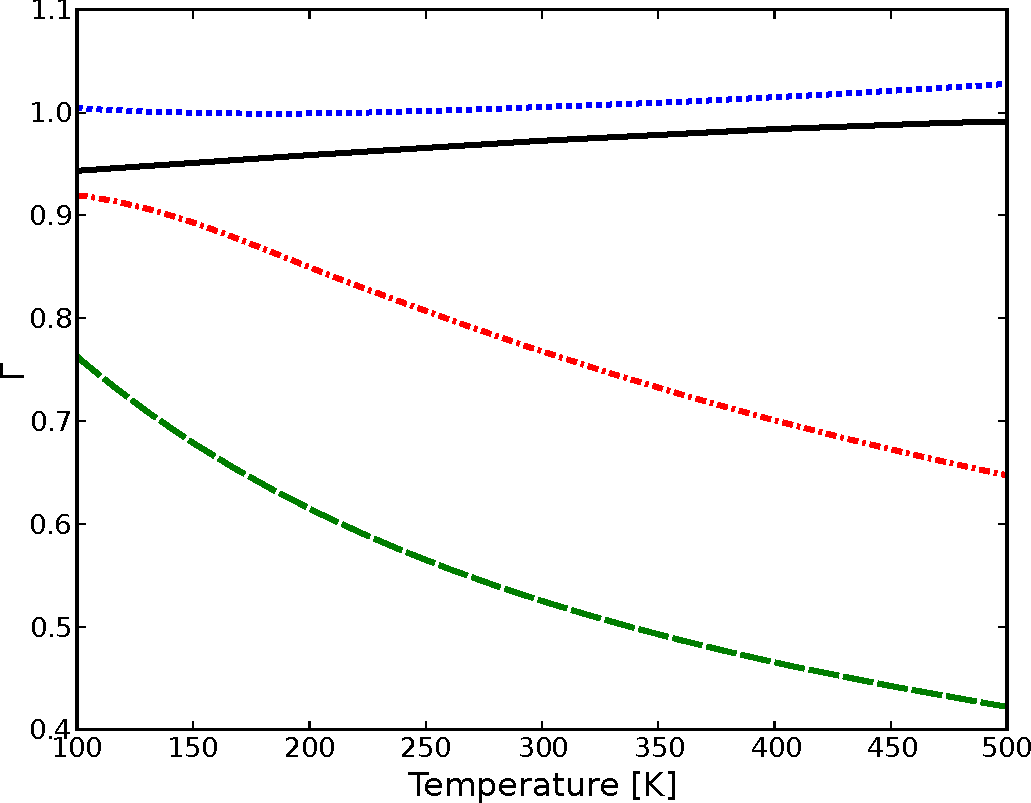
\includegraphics[width=0.5\linewidth]{figures/integral-ratios}
\caption{
The ratio, $\Gamma$, defined in \eref{eq:harmonic-correction-factor},
between the configuration integrals of the potential energy ridge shown in \fref{fig:low-barriers} and the corresponding harmonic approximations.
The black, solid, line is the ratio for the full integral, including all three concerted displacement processes.
The blue, dotted, line is the ratio when only considering the 2-atom concerted displacement.
The green, dashed, line is the ratio when only considering the 3-atom concerted displacement.
The red, dash-dotted, line is the ratio when only considering the 4-atom concerted displacement.
For the individual processes, the end points of the ridge integral are the adjacent \sap{2}s, while the full integral is done for the whole ridge.
While the harmonic approximation gives a good approximation for the total configuration integral over the whole temperature range shown, because it is dominated by the 2-atom displacement, the estimate for each of the 3-atom and 4-atom displacements is poor unless the temperature is very low.
}
\label{fig:integral-ratios}
\end{center}
\end{figure}
% ----------------------------

In the insets of \fref{fig:low-barriers}, a comparison of the atom coordinates at two adjacent \sap{1} and the intermediate \sap{2} can be seen.
In particular, the difference between the concerted 3- and 4-atom \sap{1}s is shown.
The coordinates of the two left-most atoms only change slightly while the two right-most coordinates change more, as is to be expected as the atom furthest to the right is not directly involved in the concerted 3-atom process.
The similarities in coordinates and the small \sap{2}s separating the 3- and 4-atom displacement processes indicate that a trajectory passing through the vicinity of either \sap{1} could easily end up on the product state corresponding to the other.
Dynamical trajectories started at the ridge would be needed to determine the probability of each of the product states.

% Figure 6
\begin{figure}[t]
\begin{center}
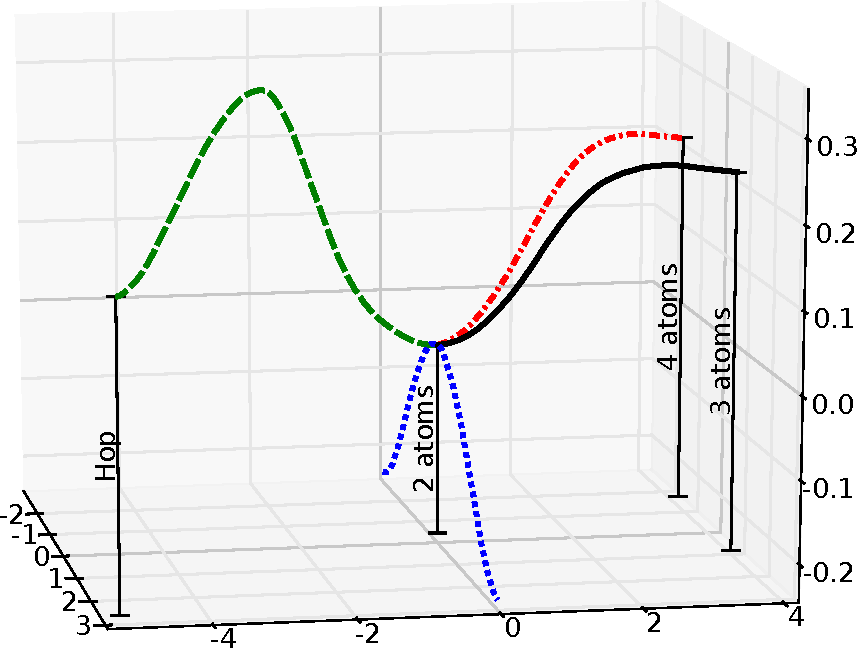
\includegraphics[width=0.5\linewidth]{figures/many-ridges}
\caption{
A schematic view (due to the high dimensionality of the system) of some of the ridges lying through the \sap{1} for 2-atom concerted displacement (the MEP is shown with blue dotted line).
The three ridges shown connect to the \sap{1}s of the hop and the 2-atom and 3-atom displacements mechanisms
The vertical bars represent the height of each of the \sap{1}s.
The figure illustrates that a \sap{1} typically lies on several energy ridges for a complex system.
}
\label{fig:multiple-ridges}
\end{center}
\end{figure}

When finding the ridge between the concerted 4-atom displacement and the hop \sap{1}s,
shown in \fref{fig:barriers-discovery},
it became apparent that a ridge does not directly connect the two.
Instead, the ridge passes through the concerted 2-atom displacement \sap{1}.
The path passes exactly through the highest \sap{2}, 
as can be verified from the calculated force, given that the climbing image algorithm is employed.
However, due to the possible corner cutting, there is no guarantee that other, lower energy, \sap{2}s along the ridge will be found exactly.
Nevertheless, if a sufficient number of images is used,
the path will give good approximation for any \sap{1}s and \sap{2}s along the ridge.
Here, the image closest to the concerted 2-atom displacement \sap{1} is found to be at a $0.004\unit{\mAA/\text{atom}}$ distance from the exact \sap{1}.
Using these coordinates in a \sap{1} searching algorithm quickly yields the exact \sap{1}.
As for the lower \sap{2}, a second ridge calculation can be performed with the adjacent \sap{1}s as endpoints to focus on a shorter segment of the ridge with only one intermediate \sap{2},
thereby enabling the climbing image to converge exactly on the lower \sap{2}.
This is shown in \fref{fig:barriers-discovery}, where the discovered \sap{1} is used as an endpoint in a subsequent optimisation of a shorter path and, thus, the lower \sap{2} is found accurately.

% Figure 7
\begin{figure}[b]
\begin{center}
\includegraphics[width=0.5\linewidth]{figures/discovery}
\caption{
Calculated path at the ridge between the \sap{1}s for a hop and concerted 4-atom displacement.
The circles show the position of converged images (coloured circles for \sap{1}s and \sap{2}s, but gray for the rest). 
These \sap{1}s turned out not to be adjacent on a ridge and the path optimisation reveals an intermediate \sap{1}, the one for the concerted 2-atom displacement.
This illustrates how a ridge calculation could reveal new and possibly unknown transition mechanisms.
The long path is not able to accurately locate the intermediate \sap{1} and the lower energy \sap{2} due to finite resolution in the discretisation and corner-cutting.
The exact configuration of the \sap{1} can be found using a \sap{1} finding algorithm starting with the approximation obtained from the optimised path.
Then, a calculation of a shorter path, between the \sap{1}s of the 2-atom  and 4-atom displacements, locates the intermediate \sap{2} accurately (cyan circle)
The insets show an overlay of three configurations, two adjacent \sap{1}s and the intermediate \sap{2}.
The atom colours correspond to the coloured spheres of the energy ridge.
}
\label{fig:barriers-discovery}
\end{center}
\end{figure}
\end{comment}


\chapter{Coupled Hydrogen Defects in Perovskites}
\label{chap:perovskites}
\textit{This chapter describes the initial testing of the ridge mapping method for a complex energy landscape with DFT forces.}
\section{Introduction}
\label{sec:perovskites-introduction}

As a DFT test system for the ridge detection method, a system that was the subject of a recent Ph.D. thesis~\cite{nicolai-2010} in Tejs VEgge's group was chosen.
The coupled hydrogen defect in a \ce{SrTiO3} perovskite structure.~\cite{double-defect-2011}
Usage of such systems can be varied, \expand
However, in the context of this thesis it was chosen as a real world example with noisy forces to briefly test the ridge detection method.

It is of particular interest to see if the diffusional process is coupled.
This had been shown in \cite{double-defect-2011} \expand




\section{Results}
\label{sec:perovskites-results}

\bit
\item Stabilisation confirmed via dimer calculations
\item Ridge calculations performed and their results are ...
\item Ridge calculations performance on a production DFT system
\item Hard to say if medium range stabilisation takes place (outlook: do similiar calculations using larger cells)
\eit


The results of Nicolai were somewhat confirmed by performing Dimer calculations which showed that the transitions of interest (low energy barriers) were, in fact, mostly those where the \ce{H} atoms would stick close to each other.
However, medium range \ce{H}-\ce{H} interaction was impossible to get reliable results for due to the size of the calculational cell, but numerous such processes were found.

\section{DFT Ridge Calculations}
In an effort to test the ridge calculations on DFT systems, the di-proton interstitial defect in \ce{SrTiO3} perovskites~\citemiss was briefly looked at.

Picking the most relevant \sap{1}s as endpoints a few ridge calculations were attempted.
Well behaved cases converged quickly but some would get trapped near minima and spend hundreds of iterations there until the calculations were aborted.
It is unlikely that this minima-trapping behaviour is an artefact of the method itself as such things did not happen in the previous test cases.\footnote{Or did they in the difficult 3-atom vs. 2-atom concerted cases?}






\chapter{Summary}
\label{chap:summary}

\subsubsection{Metal Borohydrides}
The rotational dynamics of two metal borohydrides were investigated in detail with close collaboration to experimental work.
The results of which complemented the experimental results very well.

For $\beta$-\ce{Mg(BH4)2} only rotational events were detected, with roughly $15\%$ of the \ce{BH4} groups activating very low energy ($E_b = 0.03\unit{eV}$) $C_2$-type rotations before the rest activates their $C_2$-type rotations ($E_b = 0.05 - 0.10 \unit{eV}$).
This two-fold activation of the $C_2$-type rotations was found to be dependant on the distance between \ce{B} and its \ce{Mg}-\ce{Mg} axis.
The $C_3$-type rotations were considerably higher in energy ($E_b = 0.13 - 0.30 \unit{eV}$) and did not show the same dependence as the $C_2$-type rotations.

For $\beta$-\ce{Ca(BH4)2}, not only rotational events were detected but also longer range diffusion of hydrogen.
The rotational events have activation energies of $0.09 \unit{eV}$ and $0.15\unit{eV}$ for the $C_3$- and $C_2$-type rotations, respectively.
As for the long range diffusion, many processes were considered but the only one with any significant similarities to the, very scarce, experimental data was that of a \ce{H2}-interstitial.

\subsubsection{Ridge Mapping}
In order to map ridges of functions\footnote{Steepest descent paths between first and second order saddle points.} a method was developed.
By transforming concave regions into convex ones, the dimer algorithm maps first order saddle points to minima and ridges to minimum energy paths\footnote{or path of least resistance.} (MEP), with regards to the gradient.
Using this transformation to iteratively converge a trial path to the ridge is then achieved using the nudged elastic band (NEB) algorithm for finding minimum energy paths.
Due to numerical instabilities, an artificial method for stabilisation was added to the NEB-type part of the algorithm.
This stabilisation leads to deviations in the final path --- only the path, not the second order saddle point ---
Effort to leave out or minimise this stabilisation part of the algorithm were discussed along with a discussion on the reduction of the numerical instabilities introduced by an inaccurate ridge$\rightarrow$MEP mapping.
However, these discussions lacked proper testing due to insufficient time and can, thus, only be considered as an extended and detailed outlooks.

In the context of theoretical reaction rate chemistry, the ridge method was applied to validate the reaction rates offered by the harmonic approximation to transition state theory.
Furthermore, in cases where the harmonic approximation was found lacking, a rough correction factor was offered by calculating the ratio between configurational integrals of the ridge and the harmonic energy profile.

For the \ce{Al} adatom on the \ce{Al}(100) surface system, the lowest energy mechanisms for diffusion were investigated, the hop over a bridge site and the non-intuitive concerted motion of several atoms, 2, 3 and 4.
Calculation of the ridges between each pair showed that the harmonic approximation held its ground for the lowest energy mechanism, the concerted motion of 2 atoms, and the hop, while it was found to be severely lacking for the more populous concerted motion mechanisms.
The correction factor for the latter was found to be significant.
It was also found that the ridge between the 3 and 4 atom concerted saddle points on the one hand and the hop saddle point on the other, are separated by the 2 atom concerted saddle point.
In this way finding novel mechanisms is possible using the ridge method, similarly to how the NEB method locates new minima.

The \ce{Al} system was modelled with the embedded atom method which offers gradients that are clean from numerical noise.
The dimer algorithm requires well behaved gradients since it relies heavily on finite difference methods for estimating derivatives.
In order to test this dependence, DFT calculations on the \ce{SrTiO3} perovskite system with a coupled hydrogen defect were performed.
Due to time restrictions, only a handful of ridge calculations were attempted.
Half of which were successful and found 2 low lying \sap{2}s near processes where a hydrogen defect atom would jump between neighbouring oxygen atoms.
The other half of the ridge calculations were unsuccessful and the path ended up lying near MEPs instead of ridges.
This behaviour is unexplained and requires further research.
However, there is no reason to suspect the method itself as the culprit as these flaws were not present in the other test systems.

\section{Outlook}
\label{sec:summary-outlook}

\bit
%\item DFT ridges
%\item How ridge calculations interact with different types of saddle points (such as those with $H = \vect{0}$, SPs which are also points of inflection or turning points)
%\item Rigorous performance study.
\item Discover the limit of how low \sap{2} can be with regards to \sap{1}. i.e. confirm the $5\kB T$ stuff.
%\item Use ridges to create full transition states with the dimer as normal to a hyperplanar segment
\item Catalytic Selectivity
\item Extend to Quantum HTST
\eit

\paragraph{A More Precise Ridge}
A detailed outlook as to further development of the ridge detection algorithm was presented in \fref{chap:erm}
Two efforts to reduce corner cutting on the ridge were discussed.
First by introducing a dual tangent scheme in order to minimise instabilities and remove the need for a perpendicular spring force component.
Introducing a second tangent to which the minimum mode would be perpendicular at all times.
This second tangent would be a more precise representation of the ridge than the previous tangent which is focussed at numerical stability for the MEP detection part of the algorithm.
The suggested implementation was a central difference one but a more elaborate spline implementation should also be considered.
The second effort at reducing corner cutting was by iteratively removing the perpendicular component of the spring force.
It is unclear if this second scheme is needed, should the dual tangent scheme be successful.
Both of the schemes were tested on simple systems and showed great promise but further testing and development are needed.

\paragraph{Transition State Theory}
Using the energy ridges to detect non-harmonic transitions is presented in the thesis and a correction factor is even suggested.
However, a more complete transition state rate built from the energy profile of the ridge directly is a certainly a worthwhile topic.
Furthermore, stitching together a transition state from hyperplanar segments, at each image, normal to the minimum mode is a natural progression.
Such a transition state could even be generated in a variational way, where the number of images would serve as the variational parameter in lieu of the transition state itself.

\paragraph{DFT Ridges}
DFT calculations of ridges were only moderately successful.
Investigating the reasons for this \expand \tred{(depends on the Perovskites chapter)}

\paragraph{Performance}
The performance of the ridge method was not investigated in any detail.
Subsequently, the performance was not optimised.
Such studies should be performed.

\paragraph{Application}
Only a single application was studied in detail.
Further applications could include \expand 





% Create the bibliography
\newpage
\addcontentsline{toc}{chapter}{Bibliography}
\bibliography{thesis}

% Input the papers
% Using pdfpages strips all links from the pdfs. There is a package called pax that restores some (all?) of the links. Check it out if you have the time.
\part{Papers}
\label{part:papers}

\appendix
% Hack the "Chapter" names
%\newcommand{\appchapter}[1]{\let\oldthechapter\thechapter
%  \renewcommand{\thechapter}{Paper \oldthechapter}
%    \chapter{#1}\let\thechapter\oldthechapter}

%\appchapter{Hydrogen Rotational and Translational Diffusion in Calcium Borohydride from Quasielastic Neutron Scattering and DFT Calculations}
%\label{pap:calcium}
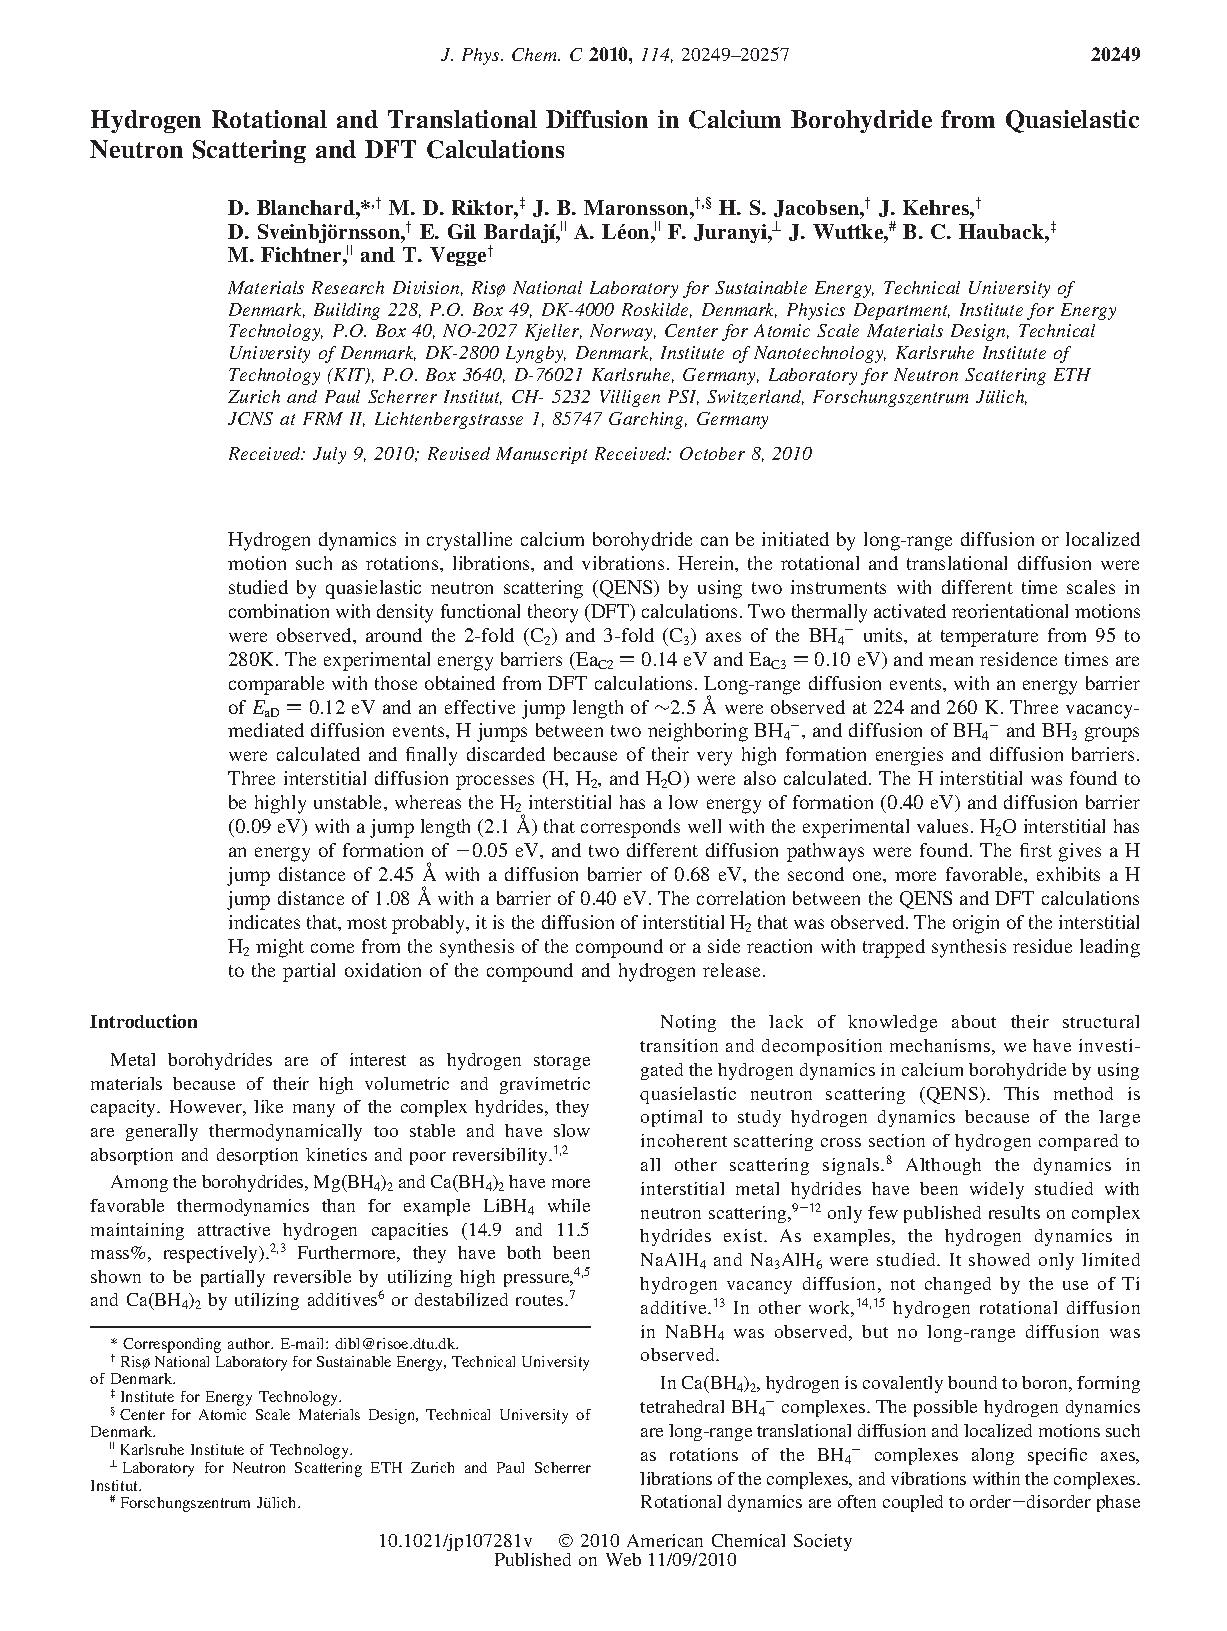
\includepdf[pages=1, addtotoc={1,chapter,0,Hydrogen Rotational and Translational Diffusion in Calcium Borohydride from Quasielastic Neutron Scattering and DFT Calculations,pap:calcium}]{papers/calcium.pdf}
%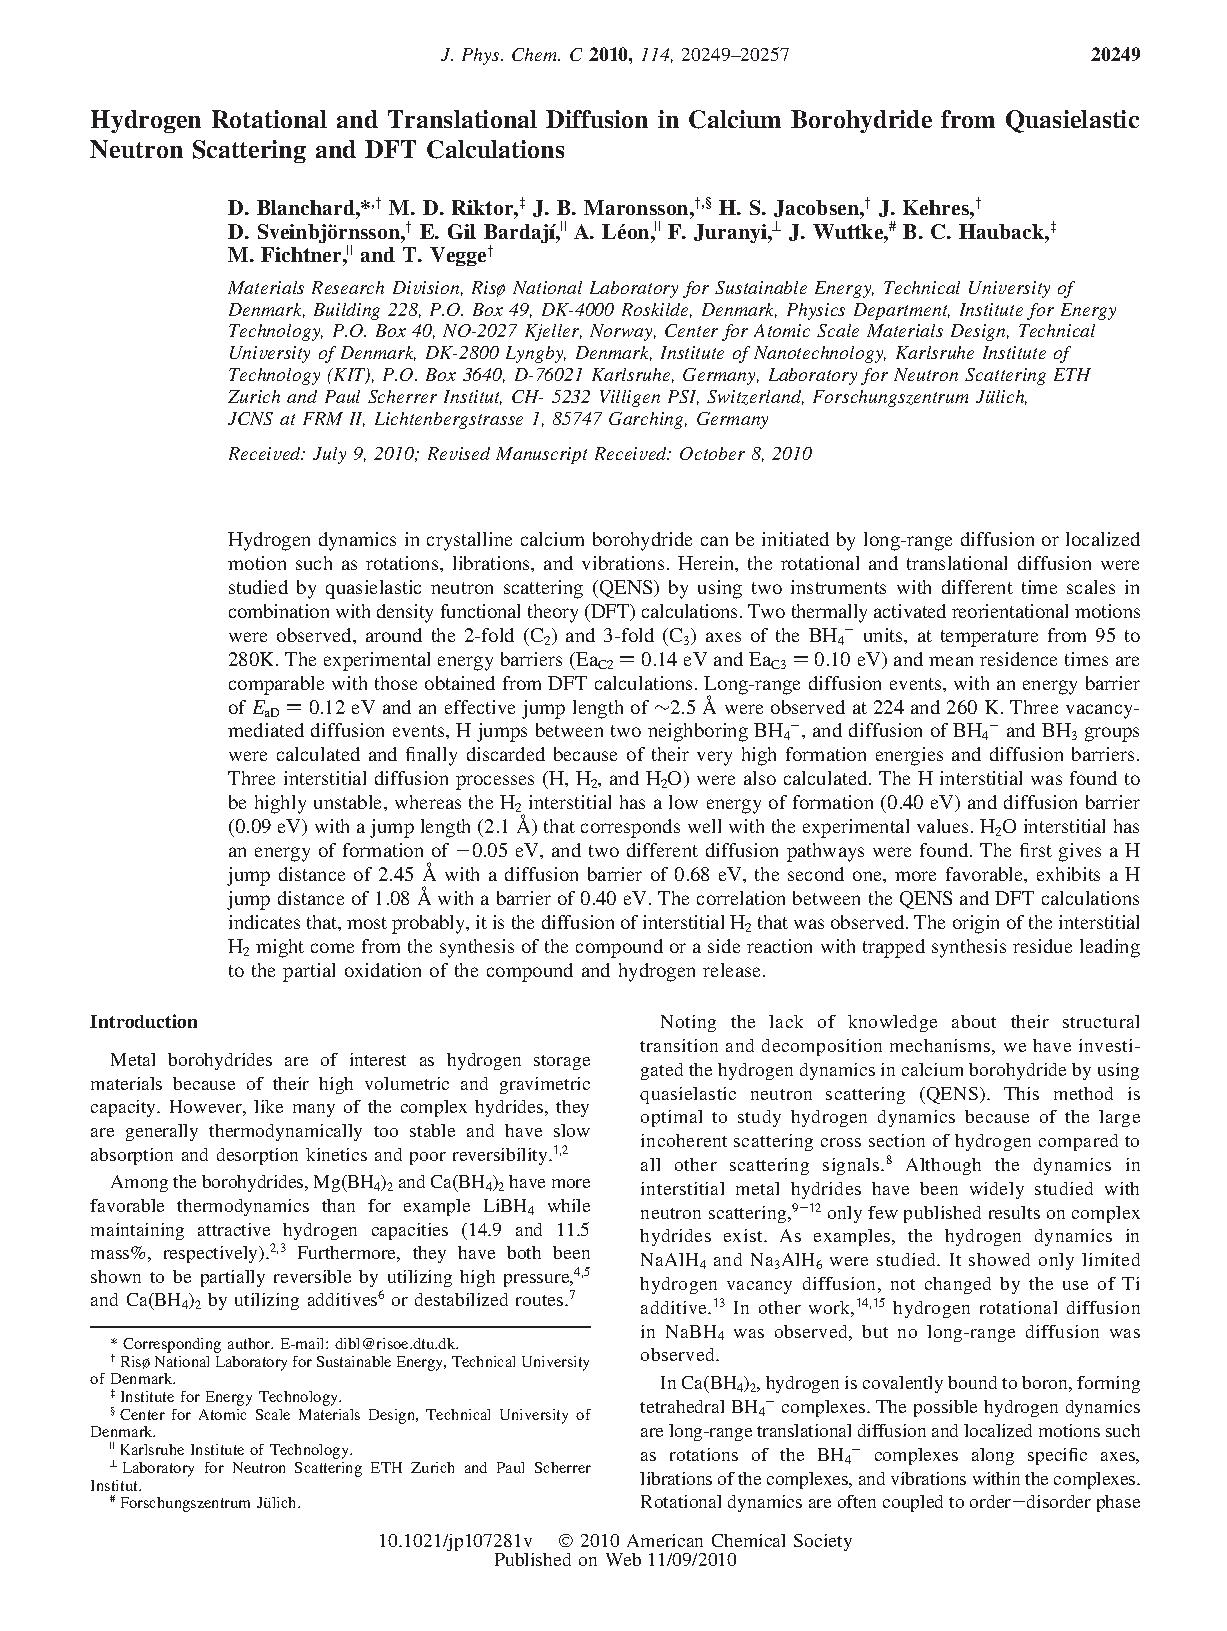
\includepdf[pages=-, openright, fitpaper, addtotoc={1,chapter,0,Hydrogen Rotational and Translational Diffusion in Calcium Borohydride from Quasielastic Neutron Scattering and DFT Calculations,pap:calcium}]{papers/calcium.pdf}

%\appchapter{Hindered Rotational Energy Barriers of \ce{BH4-} Tetrahedra in $\beta$-\ce{Mg(BH4)2} from Quasielastic Neutron Scattering and DFT Calculations}
%\label{pap:magnesium}
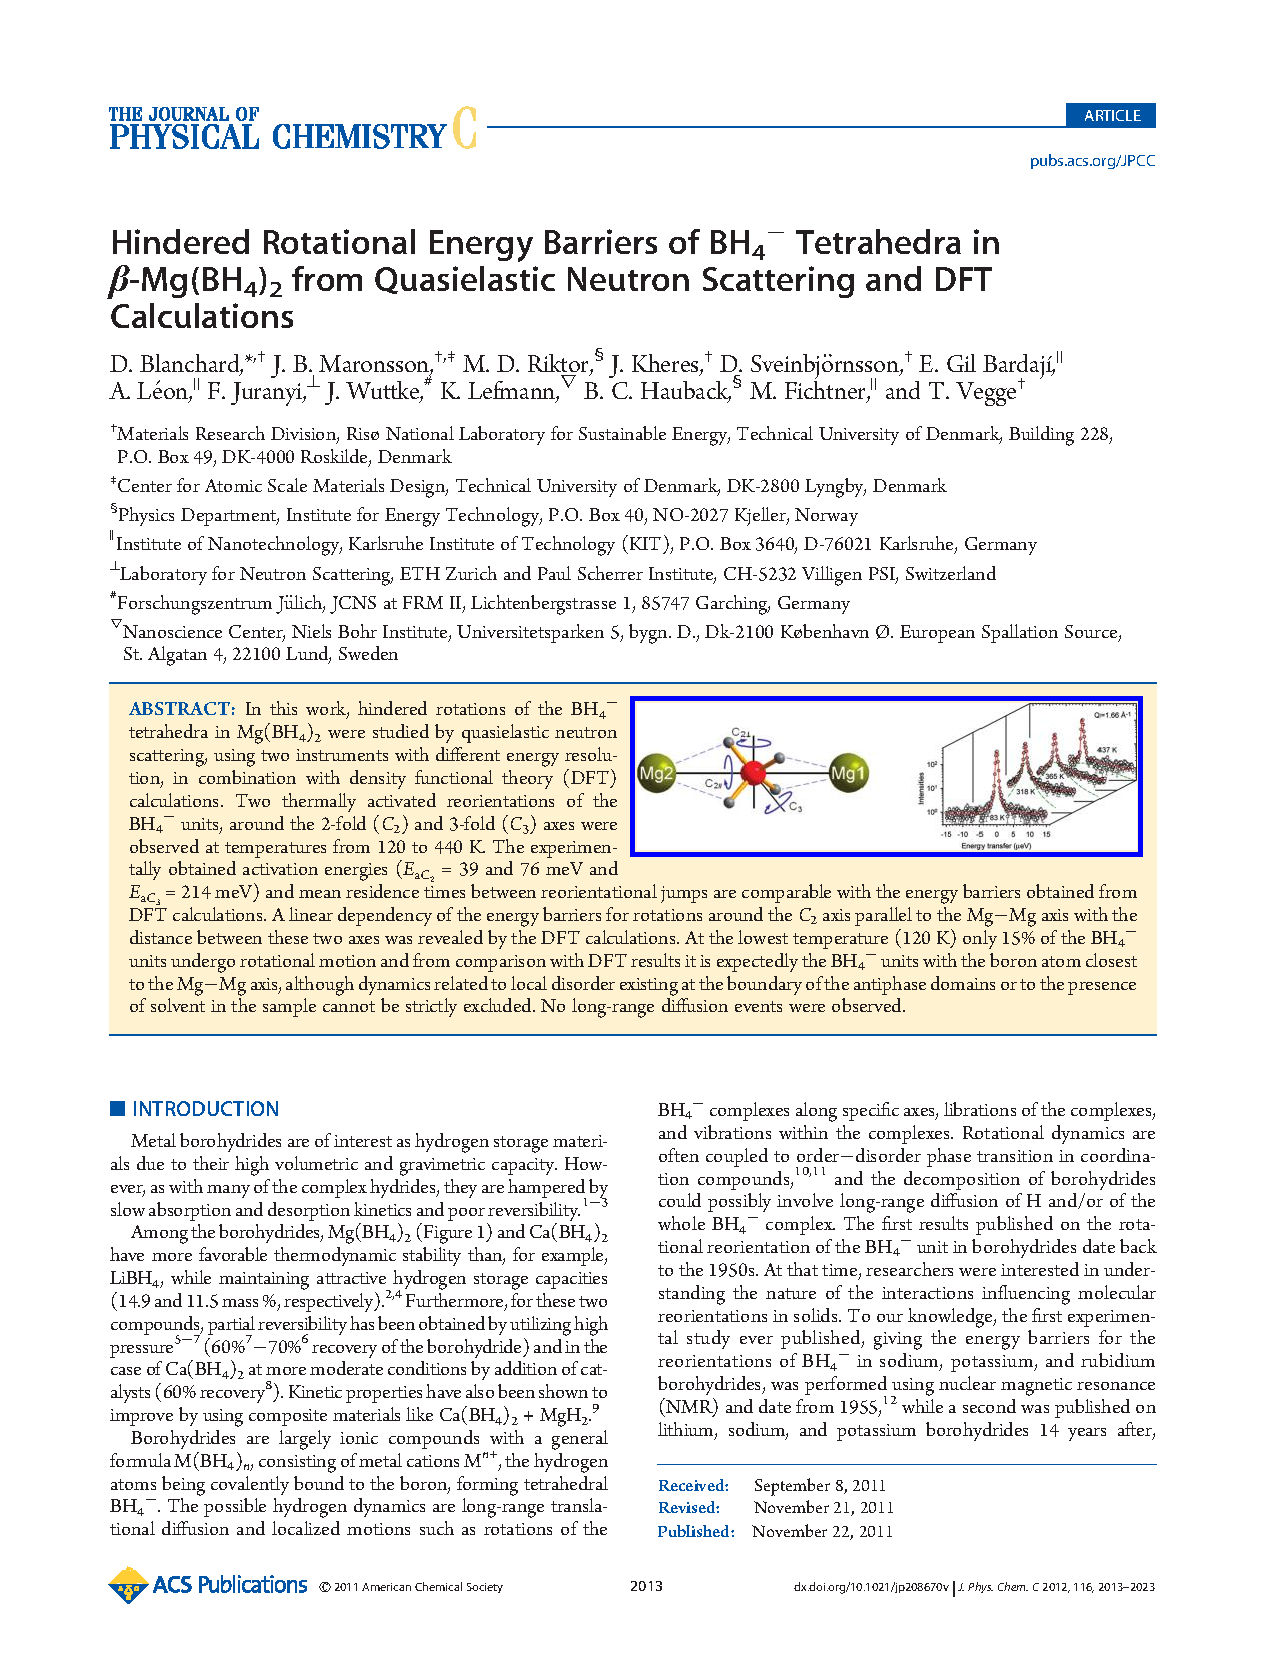
\includepdf[pages=1, addtotoc={1,chapter,0,Hindered Rotational Energy Barriers of \ce{BH4-} Tetrahedra in $\beta$-\ce{Mg(BH4)2} from Quasielastic Neutron Scattering and DFT Calculations,pap:magnesium}]{papers/magnesium.pdf}
%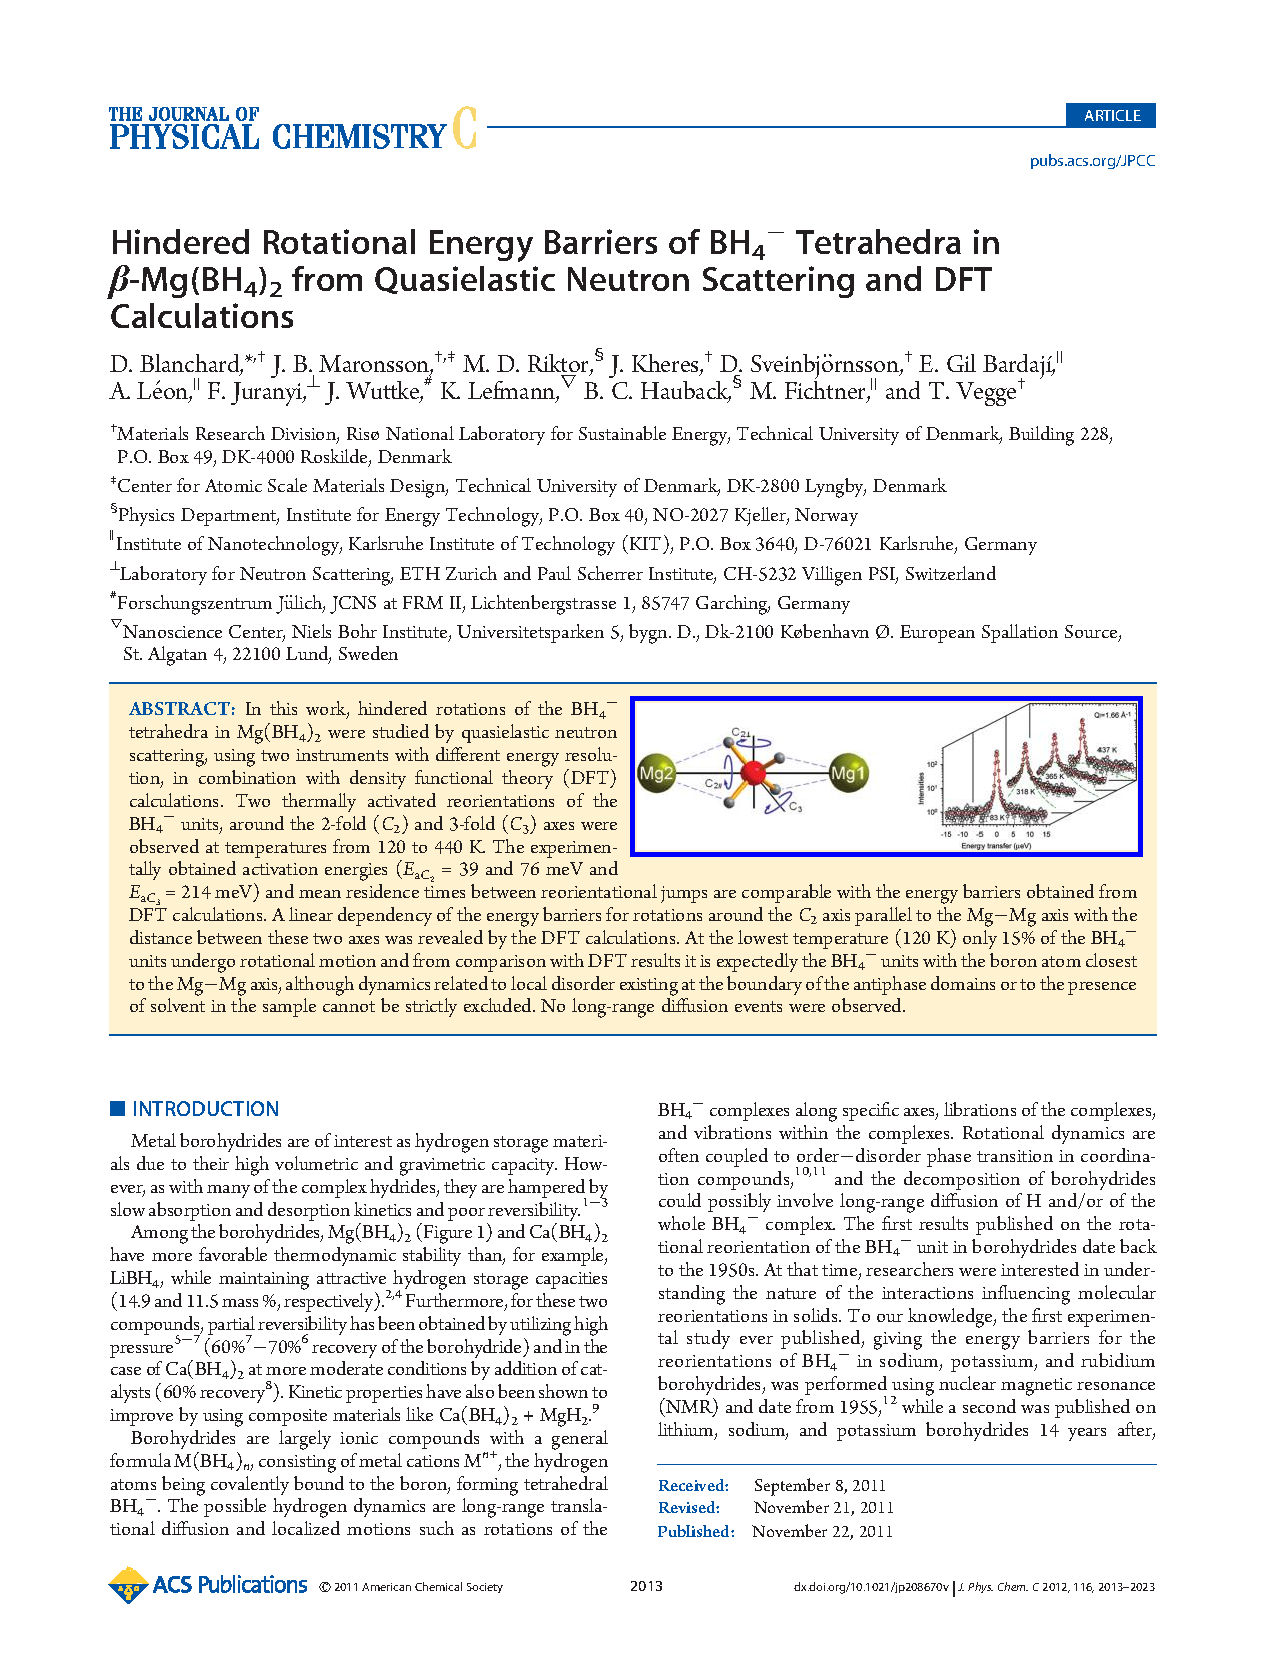
\includepdf[pages=-, openright, fitpaper, addtotoc={1,chapter,0,Hindered Rotational Energy Barriers of \ce{BH4-} Tetrahedra in $\beta$-\ce{Mg(BH4)2} from Quasielastic Neutron Scattering and DFT Calculations,pap:magnesium}]{papers/magnesium.pdf}

%\appchapter{A method for finding the ridge between saddle points applied to rare event rate estimates}
%\label{pap:second-order}
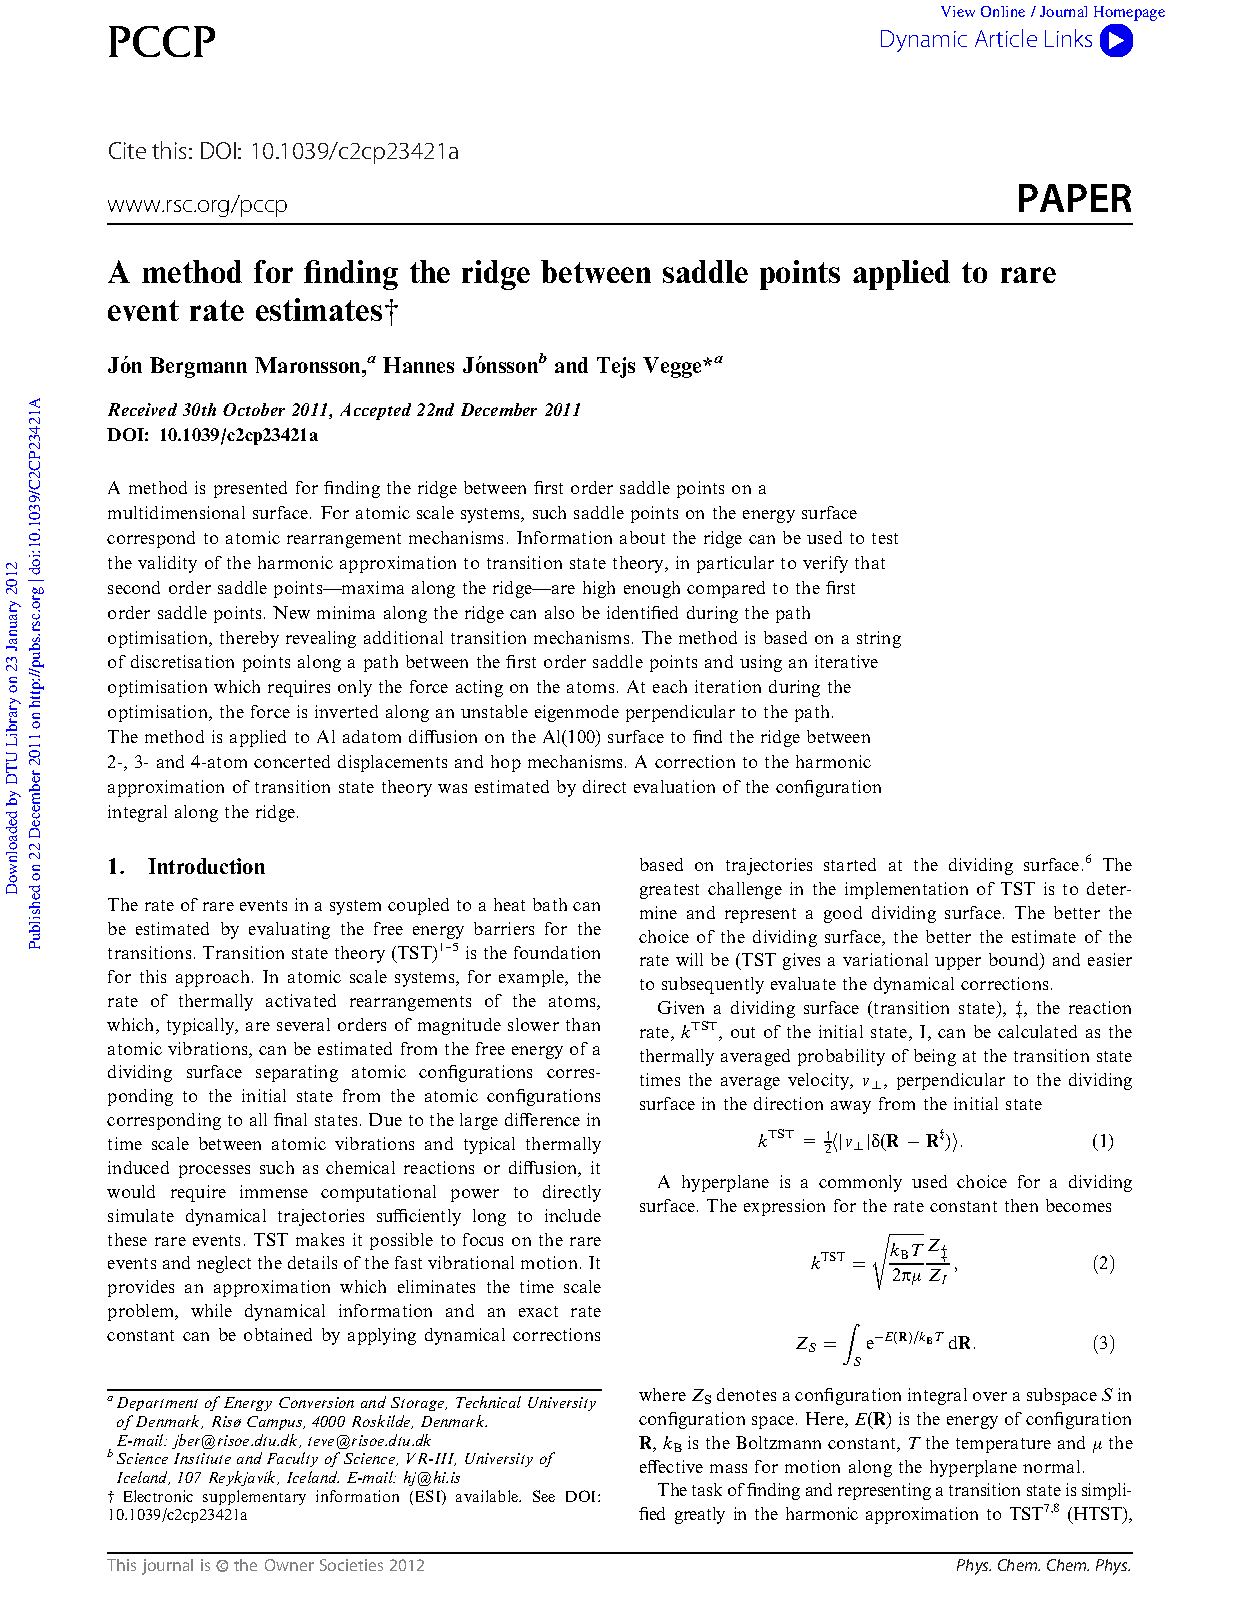
\includepdf[pages=1, addtotoc={1,chapter,0,A method for finding the ridge between saddle points applied to rare event rate estimates,pap:second-order}]{papers/second-order.pdf}
%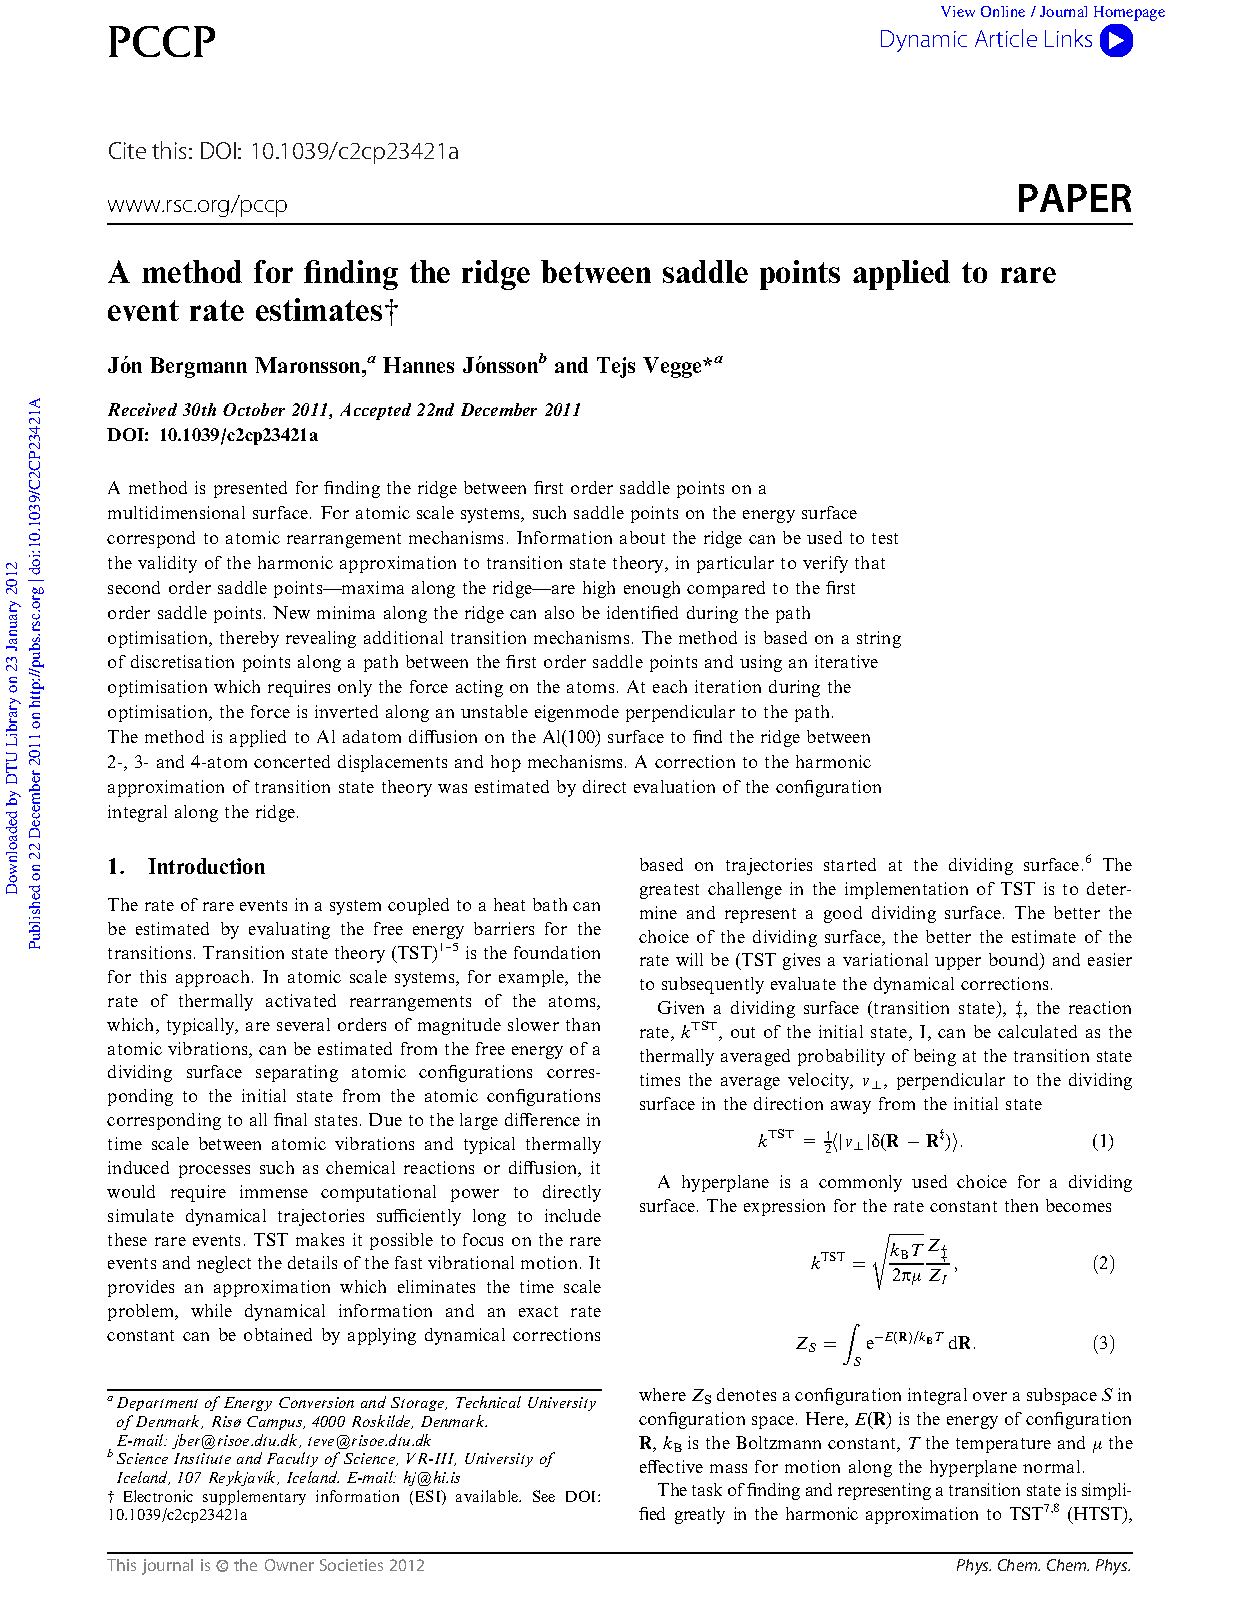
\includepdf[pages=-, openright, fitpaper, addtotoc={1,chapter,0,A method for finding the ridge between saddle points applied to rare event rate estimates,pap:second-order}]{papers/second-order.pdf}


\end{document}
